\chapter{Get Started with Elmer on Windows}

\section{Introduction}

Getting started using \texttt{Elmer} should be a smooth and easy process.  Beginners at all levels may have issues with getting started and that can be a barrier to the use of  \texttt{Elmer}.  This chapter is meant to provide help to beginners, to make it easy to start using \texttt{Elmer} and \texttt{ElmerGUI}.\\

A typical use case would be for someone with a particular application in mind that wants to find out whether \texttt{Elmer} is a suitable choice.  Being able to quickly download and run an Elmer tutorial should make the experience easy enough so the user gets an answer in a short amount of time.

%%%%%%%%%%%%%%%%%%%%%%%%%%%%

\chapter{Windows -- Download}

This chapter will discuss installing Elmer in Windows.  Windows 10 is used for these instructions.  The steps should also work with earlier versions of Windows, as long as they are 64 bits.

\section{Download Elmer}

To download the most recent release of Elmer, go to the following website:\\

\url{https://www.nic.funet.fi/pub/sci/physics/elmer/}

\begin{figure}[H]
\centering
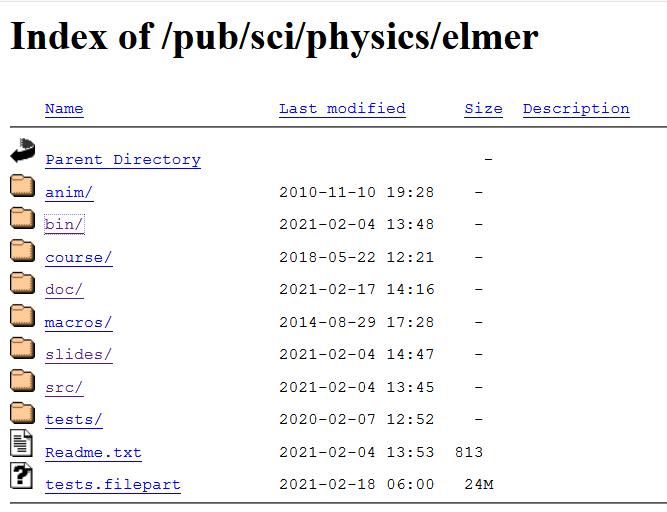
\includegraphics[width=0.8\textwidth]{elmer}
\caption{Elmer Bin Windows}\label{fg:elmer}
\end{figure}

Once on that page, there are several folders to notice, such as `bin', `doc', `slides', and `tests', as shown in Figure~\ref{fg:elmer}.  To download Elmer, click on `bin' and then `windows', and the list of Elmer installers will appear, as shown in Figure~\ref{fg:elmer-bin-win}.

\begin{figure}[H]
\centering
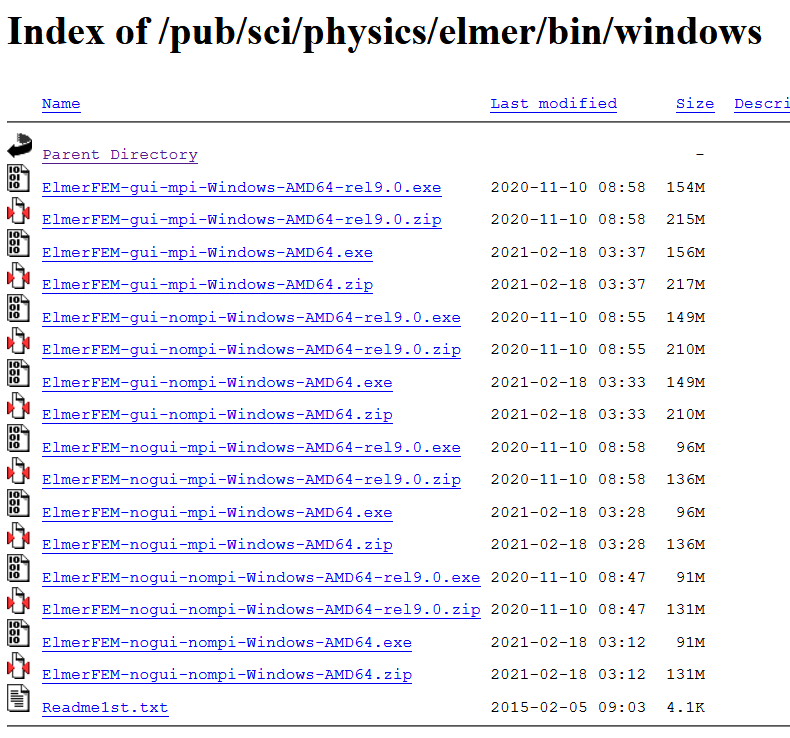
\includegraphics[width=0.9\textwidth]{elmer-bin-win}
\caption{Elmer Installers}\label{fg:elmer-bin-win}
\end{figure}

There are four main categories to select from, such as `gui-mpi', `gui-nompi', `nogui-mpi', and `nogui-nompi'.  There also some labelled with `rel9.0', which are builds of the most recent official release and should be considered as the stable builds.  The other files not labelled with `rel9.0', are the nightly builds and are the most recent builds.  The nightly builds are actually quite stable, so feel free to start with the nightly build.\\

For the first time installing Elmer in Windows, it is recommended to select `gui-mpi', and `rel9.0'.  The files with .exe extension are an installer for Windows, which is what is recommended.  So out of the entire list, we want to download this file:

\texttt{ElmerFEM-gui-mpi-Windows-AMD64-rel9.0.exe}\\

Conveniently, this is the first file in the directory listing.  If you decide to start with the nightly build, then download this file:

\texttt{ElmerFEM-gui-mpi-Windows-AMD64.exe}\\

which is the third entry in the directory listing.  If you can't decide, download both files and you can try them out separately.


\section{Download Elmer Documentation}

Return to this page, this time select `doc' for the most recent documentation for Elmer:\\

\url{https://www.nic.funet.fi/pub/sci/physics/elmer/}

\begin{figure}[H]
\centering
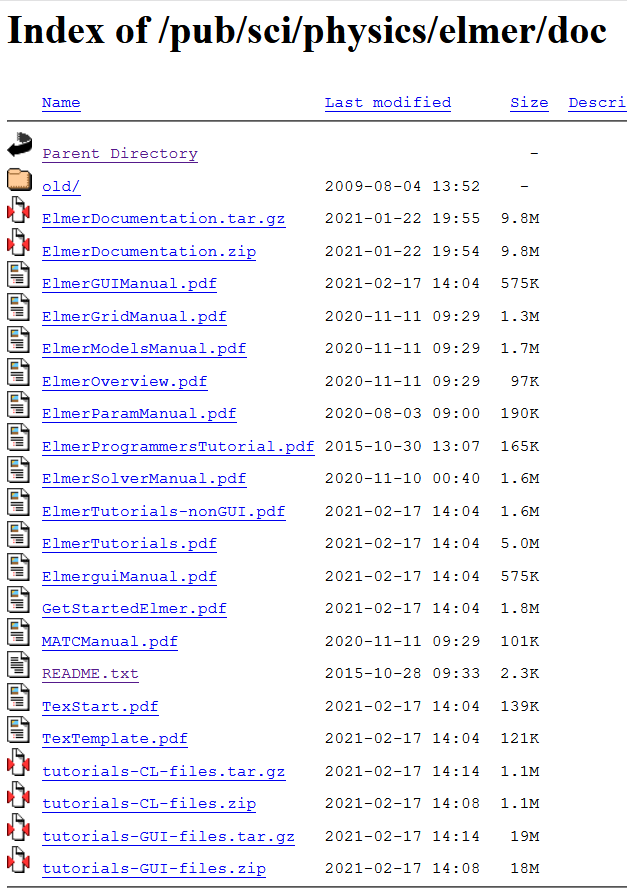
\includegraphics[width=0.8\textwidth]{elmer-doc}
\caption{Elmer Doc}\label{fg:elmer-doc}
\end{figure}

Note the two files ending in *.zip and *.tar.gz contain compressed copies of eleven out of fourteen of the documentation files.  Downloading the *.zip file should be sufficient for most Windows users to get started with Elmer.  Feel free to download all documents and all *.zip files in this directory.\\

Start with the `GetStarted' manual, which is this document.  Then look at these three documents, `ElmerTutorials' for the ElmerGUI tutorials, `ElmerGUI Manual' for instructions about ElmerGUI, and `ElmerSolverManual', which describes each solver in detail.  \\

Finally, be sure to download `tutorials-GUI-files.zip', because this zipped folder contains working examples of ElmerGUI projects, one for each tutorial.

\section{Download Paraview}

Since we are taking care of downloads, let's go ahead and get Paraview.  It's not really needed to get started with Elmer and ElmerGUI, but you'll need it at some point in the near future.  Download Paraview now, but don't install it just yet.  We'll cover installation of Paraview a little later in this discussion.\\

Go to the Download section of the Paraview website:\\

 \url{https://www.paraview.org/download/}\\

Select one of the top items, in particular a file ending in .exe, so you will download a Windows installer version.  You should now have a file like this:\\

\texttt{ParaView-5.9.0-RC3-Windows-Python3.8-msvc2017-64bit.exe}\\

On the Paraview download page, there are several other files, such as `getting started', `tutorial', that would be very useful to download.  This would be a good opportunity to download the instructions for Paraview.


%%%%%%%%%%%%%%%%%%%%%%%%%%%%

\chapter{Windows -- Install}

\section{Install Elmer}

Navigate to the folder containing the Elmer installer and the documentation zip file.  Extract the zip file to a suitable folder.  You should have selected one version of the Elmer installer by now.  The installer with \texttt{gui-mpi} will install ElmerGUI, Elmersolver, Elmersolver\_mpi, and Microsoft MPI.  This will provide the capability to run solutions serially or in parallel.  To get started with Elmer and ElmerGUI, running solutions serially is the best way to learn how to use the program.  We will cover setting up and running in parallel in a later chapter.  It is suggested to get some experience with serial solutions, then later on refer to the chapter on Parallel Solutions.\\

Double click on the Elmer installer .exe file.  The installation process should look like figures~\ref{fg:installer-1}  through figures~\ref{fg:installer-13} on the following pages.  

\begin{figure}[H]
\begin{center}
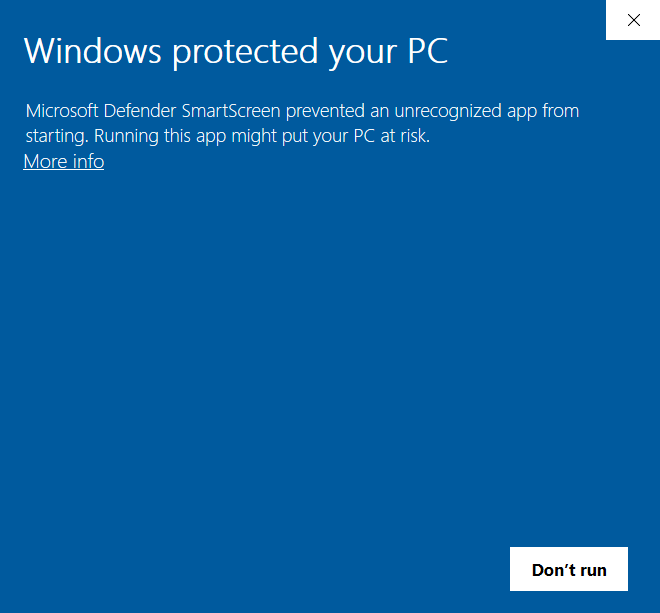
\includegraphics[width=0.48\textwidth]{installer-1}
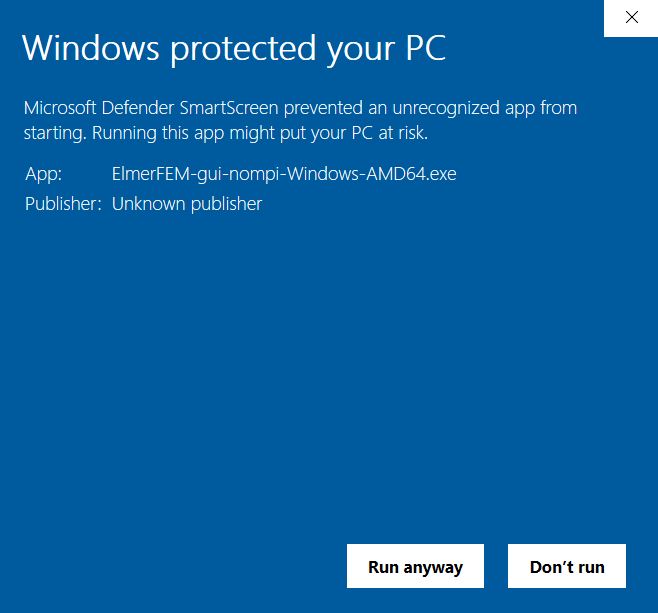
\includegraphics[width=0.48\textwidth]{installer-2}
\caption{Elmer installation, click on the More info button, then Run anyway}\label{fg:installer-1}
\end{center}
\end{figure}

You may get a blue screen while beginning the installation.  The first blue screen has a small button, `More info', that you must click on to get the second blue screen, where you will click on `Run anyway'. 

From there just take the default actions up until you reach `Install Options', where you have a chance to select adding the path to Elmer.  Be sure to click on `Add Elmer...', either for all users or for current user.  If you aren't sure, pick `for current user'.  Also put a check into the check box for `Create Elmer Desktop Icon'.  From here, take the defaults and it should properly install Elmer.\\

\begin{figure}[H]
\begin{center}
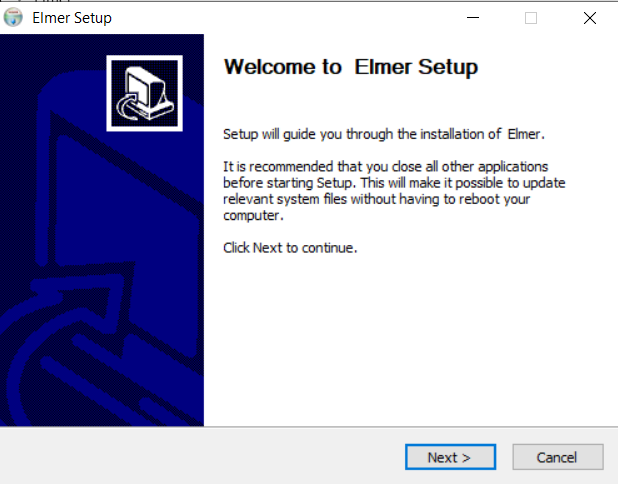
\includegraphics[width=0.45\textwidth]{installer-3}
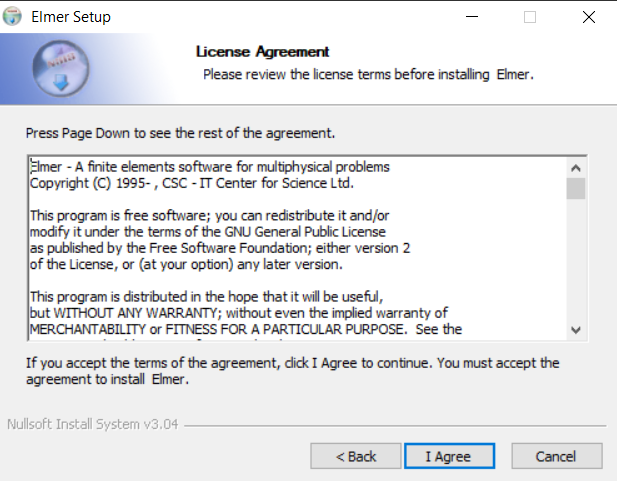
\includegraphics[width=0.45\textwidth]{installer-4}
\caption{Elmer installation, agree to the license}\label{fg:installer-3}
\end{center}
\end{figure}

\begin{figure}[H]
\begin{center}
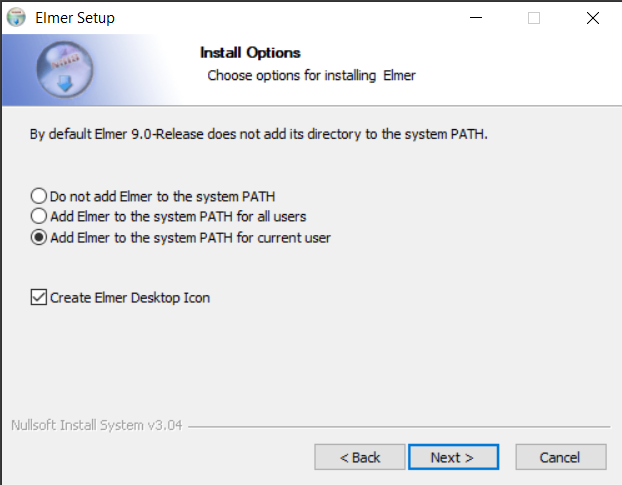
\includegraphics[width=0.45\textwidth]{installer-5}
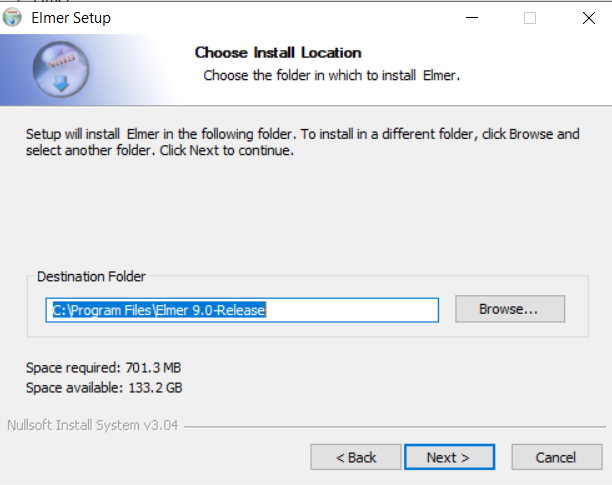
\includegraphics[width=0.45\textwidth]{installer-6}
\caption{Select Install Option: Add Elmer to the system PATH for current user}\label{fg:installer-5}
\end{center}
\end{figure}

If this is the first time installation of Elmer, be sure to select all four components.  If upgrading or reinstalling, then you can uncheck the box for `MS MPI', no need to reinstall MPI.

\begin{figure}[H]
\begin{center}
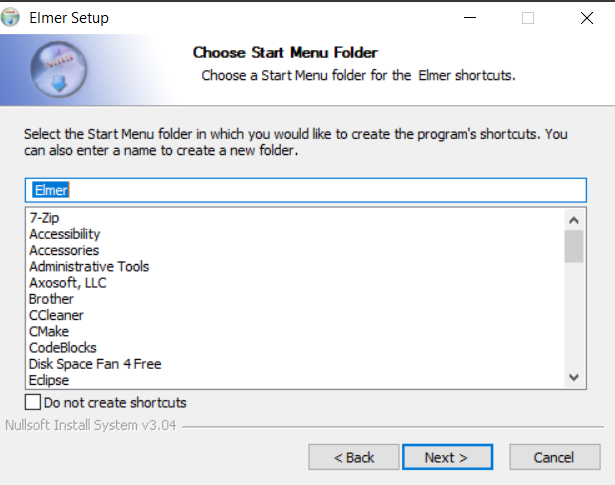
\includegraphics[width=0.45\textwidth]{installer-7}
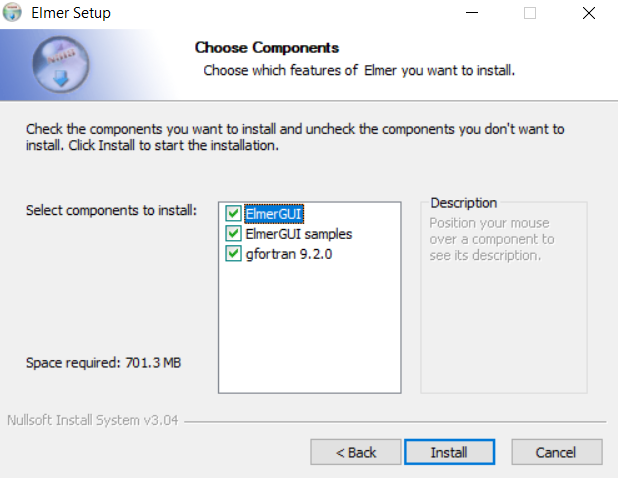
\includegraphics[width=0.45\textwidth]{installer-8}
\caption{Select Components, take the defaults}\label{fg:installer-7}
\end{center}
\end{figure}

\begin{figure}[H]
\begin{center}
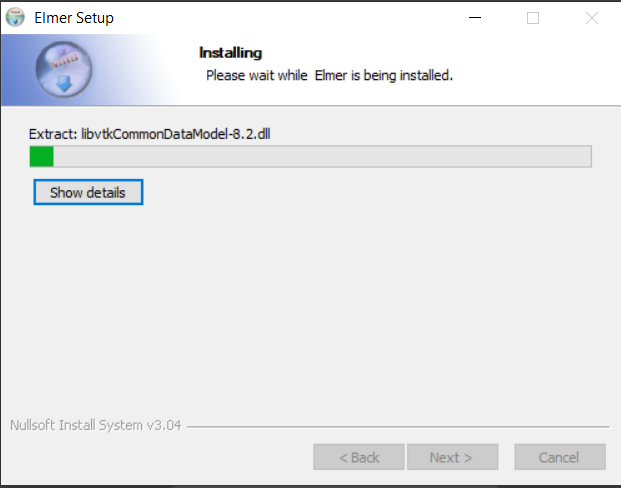
\includegraphics[width=0.45\textwidth]{installer-9}
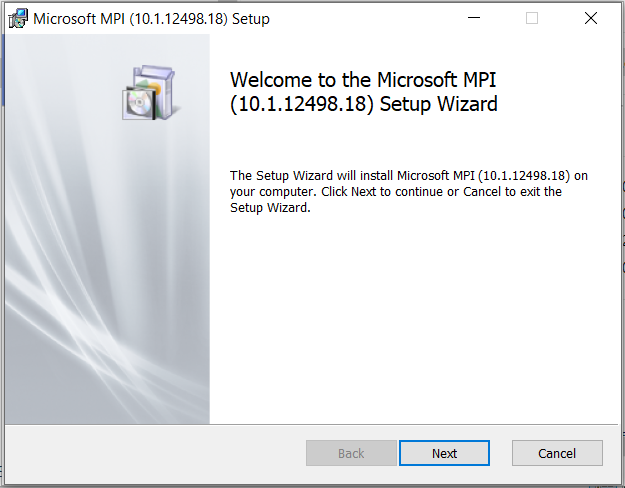
\includegraphics[width=0.45\textwidth]{mpi-1}
\caption{MPI installation occurs on first installation of Elmer}\label{fg:installer-9}
\end{center}
\end{figure}

\begin{figure}[H]
\begin{center}
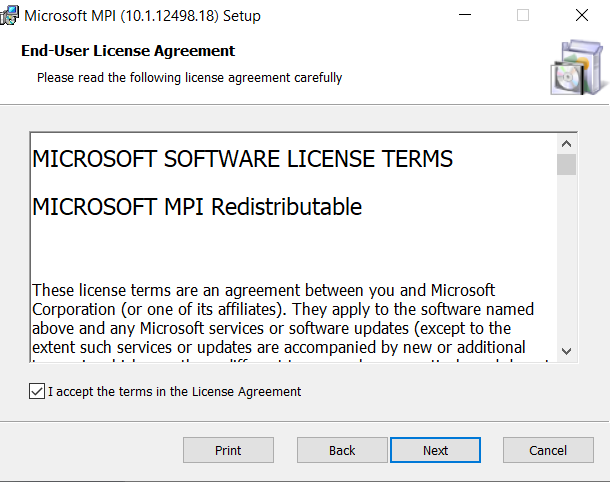
\includegraphics[width=0.45\textwidth]{mpi-2}
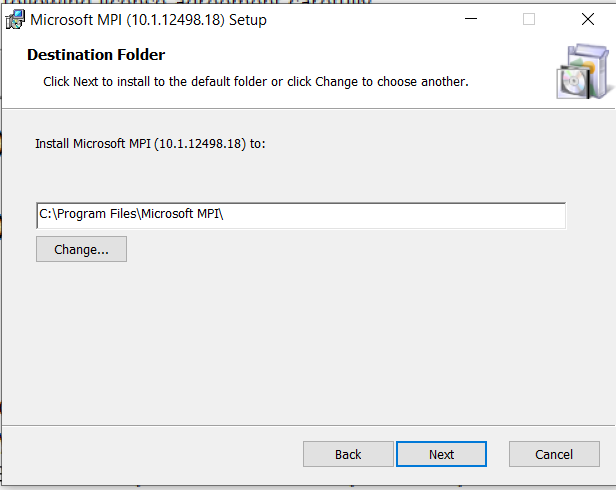
\includegraphics[width=0.45\textwidth]{mpi-3}
\caption{Agree to the license and take the default directory}\label{fg:installer-10}
\end{center}
\end{figure}

\begin{figure}[H]
\begin{center}
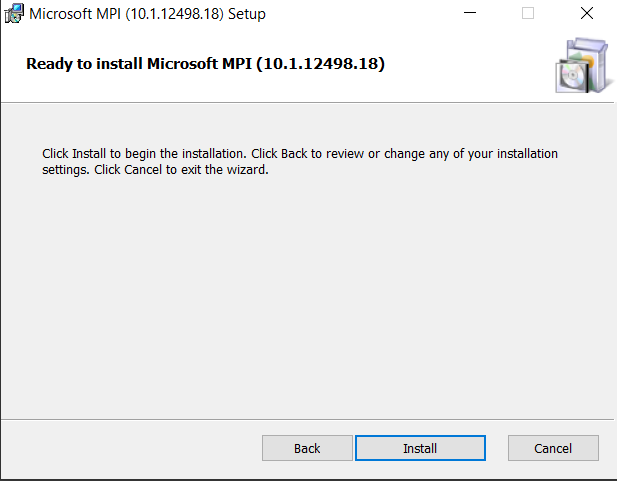
\includegraphics[width=0.45\textwidth]{mpi-4}
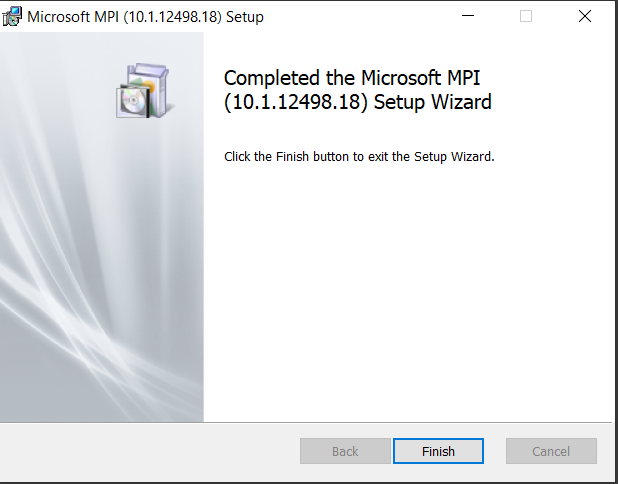
\includegraphics[width=0.45\textwidth]{mpi-5}
\caption{Complete MPI installation}\label{fg:installer-11}
\end{center}
\end{figure}

\newpage

If you see the below Figure \ref{fg:installer-12} during the installation process, don't worry, just go ahead and click on the \texttt{OK} button.  This message appears if you have previously installed Microsoft MPI, and as the notice box says, there is already a version of MPI installed.  This will happen every time you install a newer version of Elmer with MPI, regardless of whether you uninstall Elmer first, or if you just install a newer version on top of an old version.  The Elmer uninstaller doesn't uninstall Microsoft MPI, so if you want to uninstall MPI, you will have to go find the right instructions from Microsoft.

\begin{figure}[H]
\begin{center}
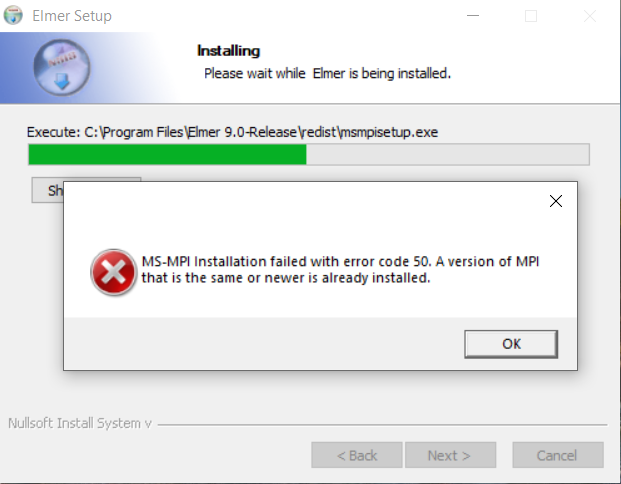
\includegraphics[width=0.60\textwidth]{mpi-6}
\caption{Don't repeat MPI installation, click on OK}\label{fg:installer-12}
\end{center}
\end{figure}

\begin{figure}[H]
\begin{center}
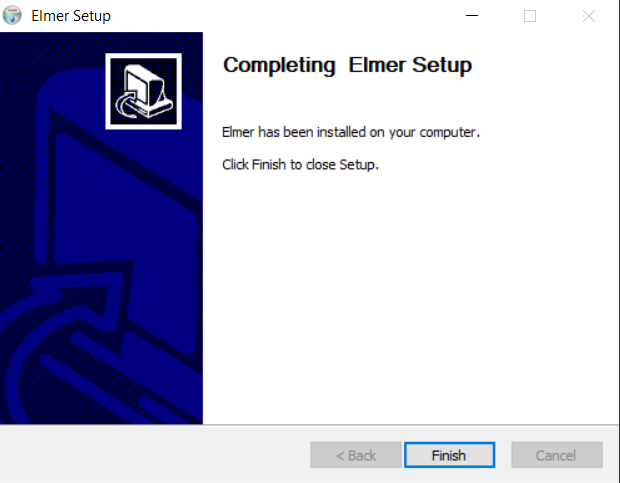
\includegraphics[width=0.60\textwidth]{installer-10}
\caption{Complete the Elmer installation}\label{fg:installer-13}
\end{center}
\end{figure}

After the installation process has finished, you should see an icon on the desktop for ElmerGUI.  Go ahead and double click on the icon to start ElmerGUI.  Please refer to the ElmerGUI manual for instructions on using ElmerGUI, and try out the first tutorial. 

Since Paraview hasn't been installed yet, after loading the first tutorial  if you click on the `Run', then on `Start Paraview', nothing much will happen.  If you hover the cursor over the flag after clicking on it, you will see in the lower left of the window the message `Unable to start Paraview'.  In the meantime, to start ElmerVTK click on the top menu bar icon `Run', then click on `Start ElmerVTK'.


\section{Install Paraview}

Navigate to the folder containing the Paraview installer.  Double click on the installer to start the installation process.  There really aren't any options that need to be selected or changed for a successful installation.  The installer won't create a desktop icon, but will create an entry in the Start menu.\\

The installer will not add Paraview to the system path, we will have to perform that step ourselves.


%%%%%%%%%%%%%%%%%%%%%%%%%%%%

\chapter{Windows -- Path to Paraview}

\section{View the Path to Elmer}

If we set the path to Paraview, then ElmerGUI will be able to start Paraview from inside of ElmerGUI.  In other words, with a proper path setting, clicking on `Start Paraview', will start Paraview and load the current .vtu file, if it exists.

To set the path after installing Paraview, click on `Start', then `Settings'.  As shown in figure~\ref{fg:path-1}, start typing in the search box `environment', then select the result for `Edit environment variables for your account'.  

\begin{figure}[H]
\begin{center}
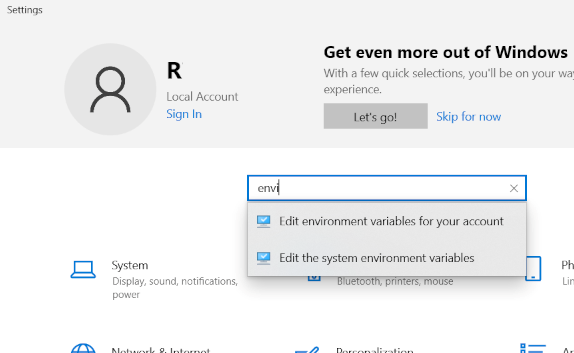
\includegraphics[width=0.95\textwidth]{path-1}
\caption{Settings: Search for Environment variables}\label{fg:path-1}
\end{center}
\end{figure}

\newpage

As part of the operation of the Elmer installer, the path to Elmer will be created.  Let's verify that the path to Elmer exists.  Open the window then select `path' and click `edit', as shown in figure~\ref{fg:path-2}.   Notice Elmer is at the bottom of the list, since it was the most recently installed program.  

\begin{figure}[H]
\begin{center}
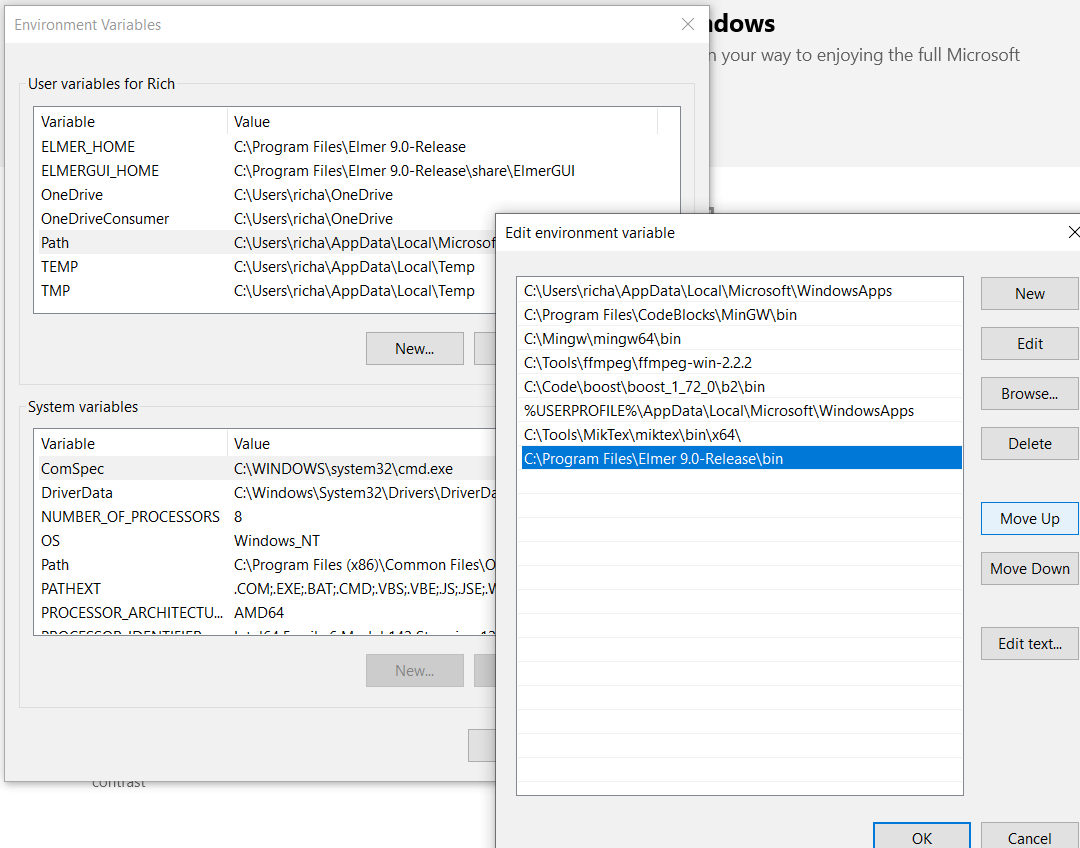
\includegraphics[width=0.9\textwidth]{path-2}
\caption{Path to Elmer installation}\label{fg:path-2}
\end{center}
\end{figure}

\section{Add the Path to Paraview}

While you have the path variable open for editing, click on `new', and enter the path to Paraview.\\

One way to find out what is the exact path to your installation of Paraview is as follows.  Open File Explorer and select your system drive, such as C:, then open Program Files and then open the folder for Paraview.  Next open the bin folder and you will see an entry for Paraview.exe, this is the location that you want to enter into the path, as shown in figure~\ref{fg:path-3}.

\begin{figure}[H]
\begin{center}
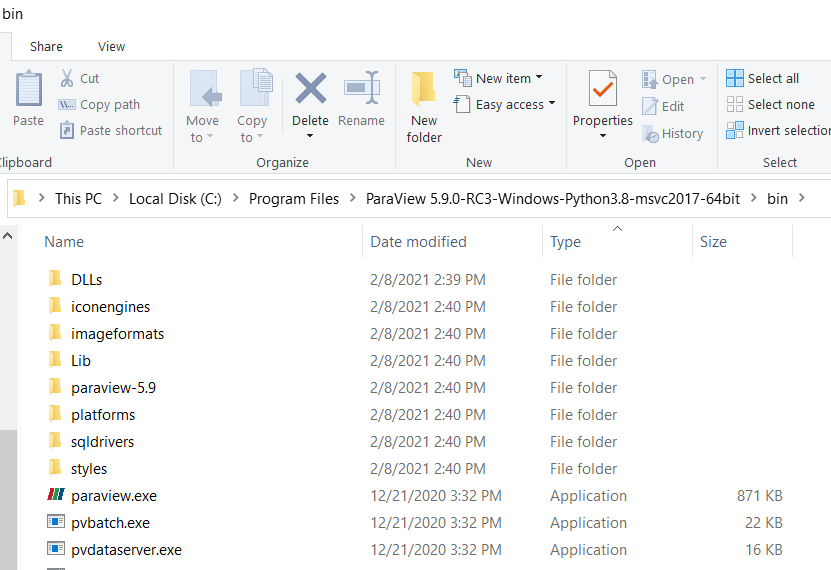
\includegraphics[width=0.75\textwidth]{path-3}
\caption{Select the path to Paraview}\label{fg:path-3}
\end{center}
\end{figure}

Copy the path to the bin folder into the new path environment variable.  Tip: you can actually copy and paste the path from File Explorer into the new environment path variable, as shown in figure~\ref{fg:path-4}.\\

\begin{figure}[H]
\begin{center}
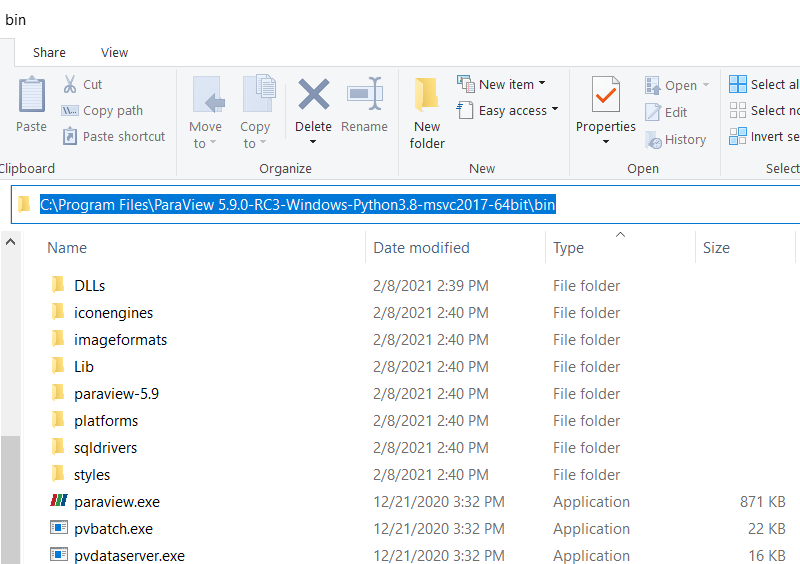
\includegraphics[width=0.75\textwidth]{path-4}
\caption{Copy the path to Paraview}\label{fg:path-4}
\end{center}
\end{figure}

Not completely necessary, but just suggested, you may want to move the path to 
Elmer up to the top of the list, as shown in figure~\ref{fg:path-5}.\\

Finally, move the entry for the path to Paraview up to just under the path to Elmer, as shown in figure~\ref{fg:path-5}.  Click `ok' to save your edits, then exit settings.

\begin{figure}[H]
\begin{center}
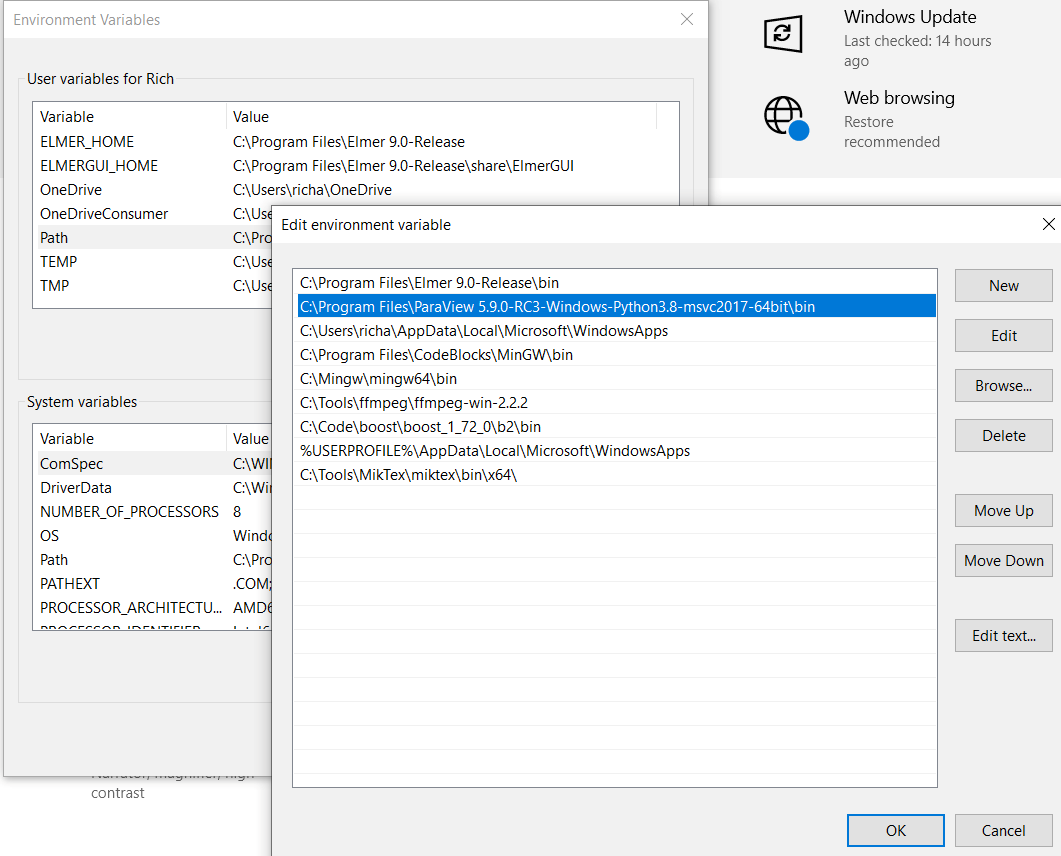
\includegraphics[width=0.9\textwidth]{path-5}
\caption{Create new path to Paraview}\label{fg:path-5}
\end{center}
\end{figure}

\section{Start Paraview from within ElmerGUI}

Open ElmerGUI, and click on 'Run', then `Start Paraview', you should see a pop up window that says `Paraview Starting', followed by Paraview actually starting.  If you see an output window containing a red statement like `critical: In unknown, line 0', don't worry, it just means there wasn't a valid .vtu file found.  Run a tutorial, or find a valid .vtu file, and try again, Paraview should load the .vtu file and display a blank grey screen.

%%%%%%%%%%%%%%%%%%%%%%%%%%%%

\chapter{Introduction to Paraview}

If you have loaded a valid Elmer .vtu file, upon opening Paraview you will see a blank grey screen, and many small icons, as shown in Figure~\ref{fg:paraview-2}.

\begin{figure}[H]
\begin{center}
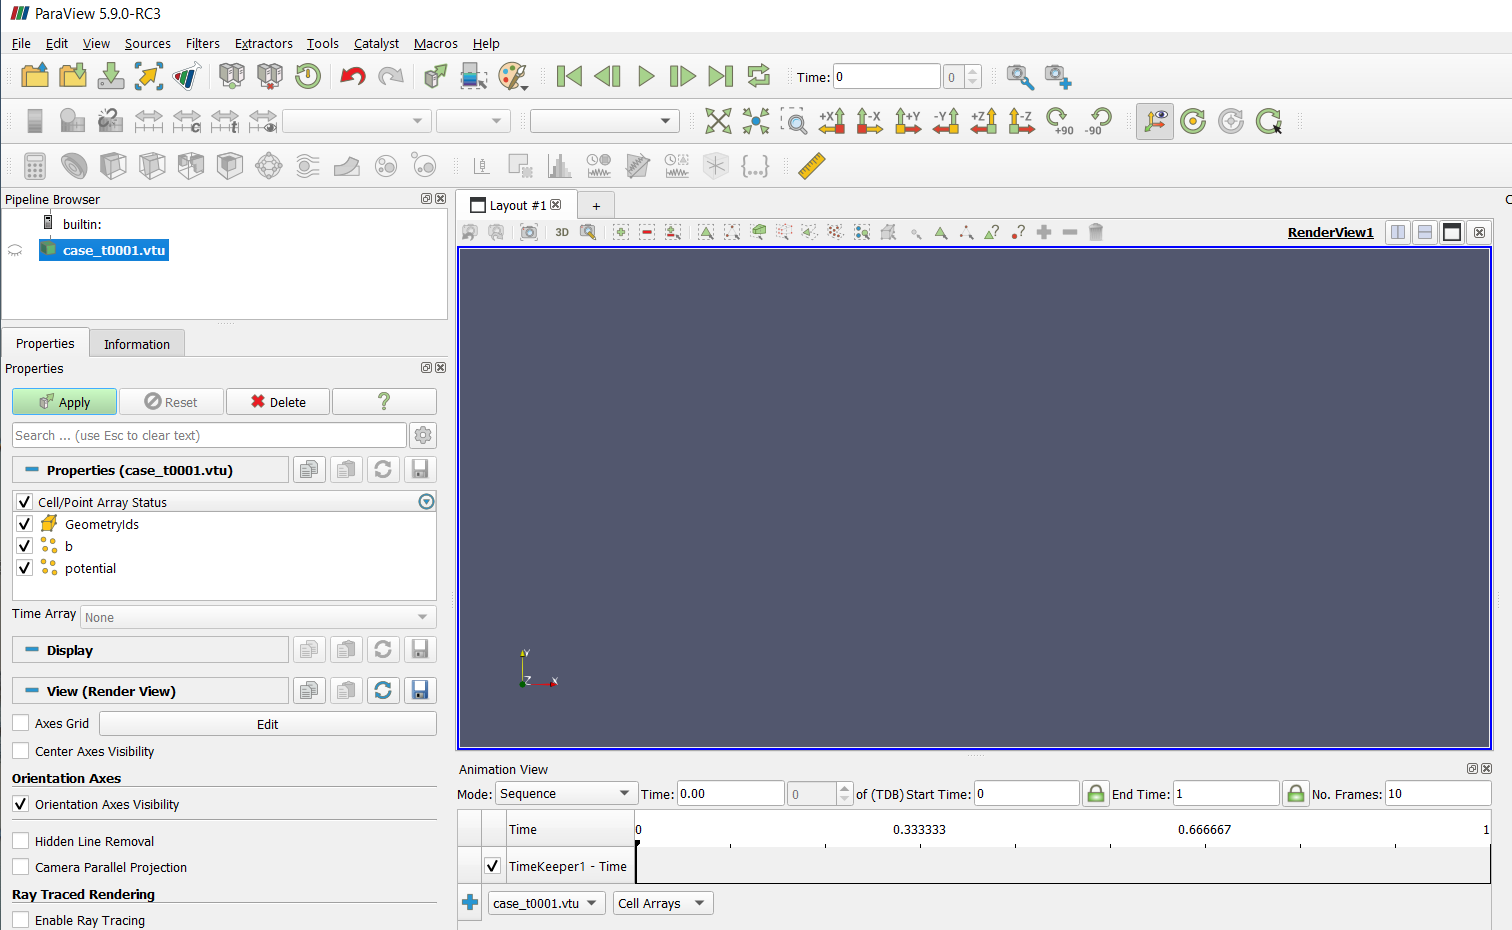
\includegraphics[width=0.58\textwidth]{paraview-2}
\caption{Initial Paraview screen}\label{fg:paraview-2}
\end{center}
\end{figure}

On the left side of the screen, as shown in Figure~\ref{fg:paraview-4}, near the middle is a light green button `Apply'.  Click on that button and the geometry will appear.

\begin{figure}[H]
\begin{center}
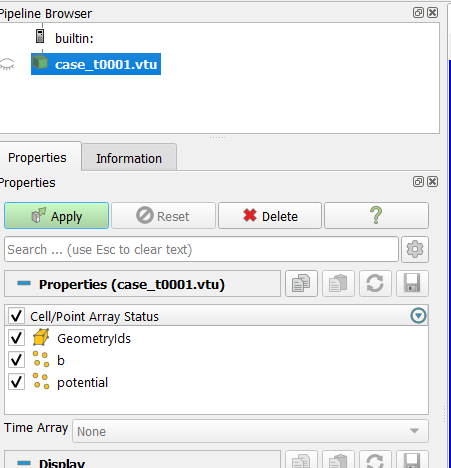
\includegraphics[width=0.38\textwidth]{paraview-3}
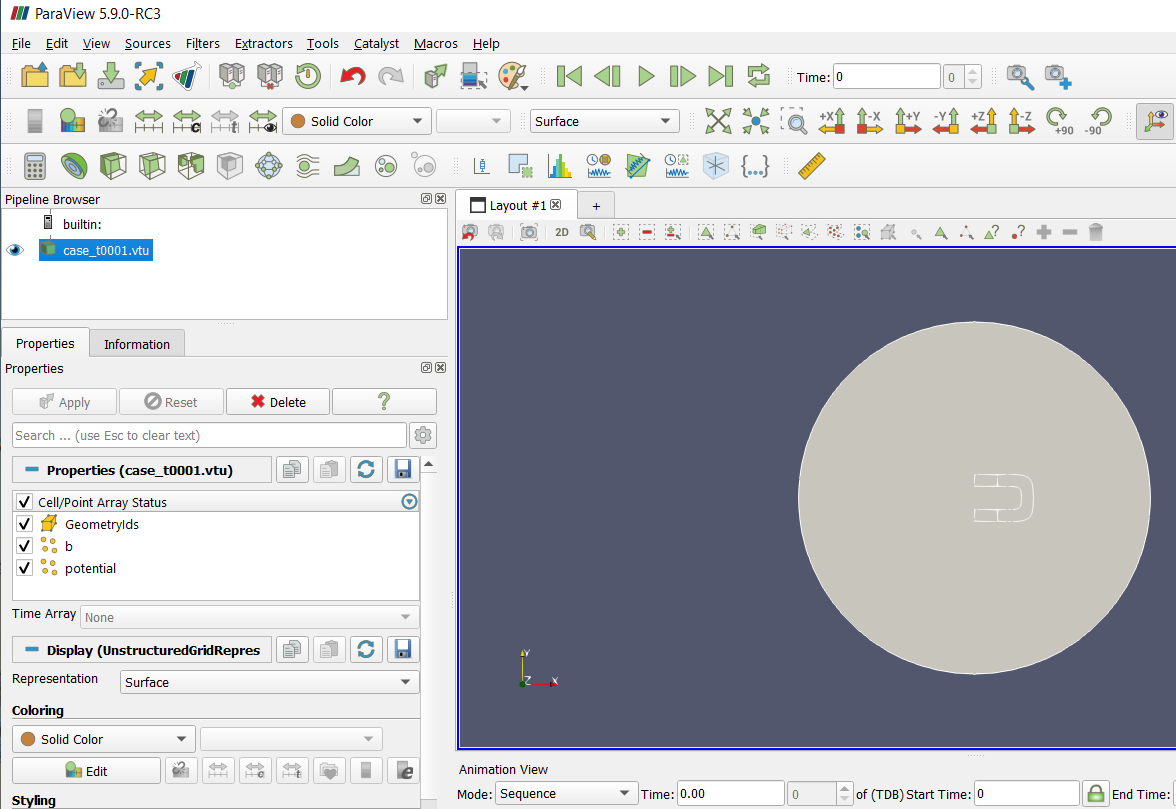
\includegraphics[width=0.57\textwidth]{paraview-4}
\caption{Left side click Apply, right side geometry appears}\label{fg:paraview-4}
\end{center}
\end{figure}

\newpage

Next, look on the left side below the window showing the variables, as shown in Figure~\ref{fg:paraview-5}, for a box labelled `Coloring'.  Click in that box for a drop down selection, pick `potential', then click `Apply'.  The potential will appear superimposed on the geometry, along with a color bar with the range of the potential.

\begin{figure}[H]
\begin{center}
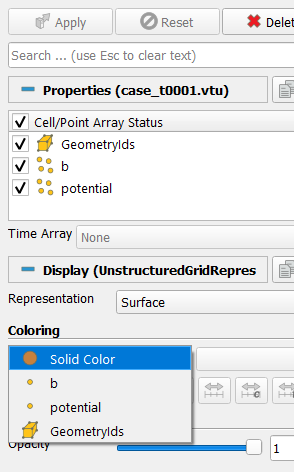
\includegraphics[width=0.3\textwidth]{paraview-5}
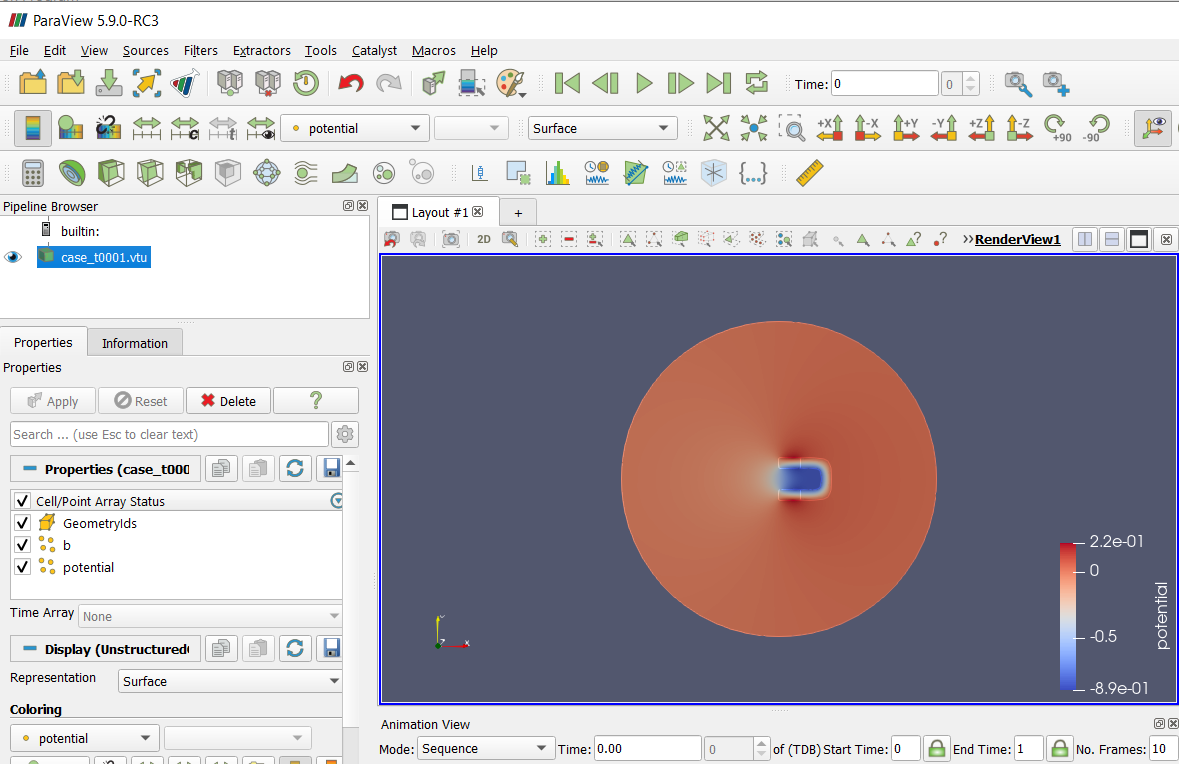
\includegraphics[width=0.68\textwidth]{paraview-6}
\caption{Initial Paraview screen}\label{fg:paraview-5}
\end{center}
\end{figure}

That is a very basic introduction to Paraview.  For more information, refer to the  Paraview website.

%%%%%%%%%%%%%%%%%%%%%%%%%%%%

\chapter{Introduction to ElmerVTK}

ElmerGUI is equipped with ElmerVTK, a graphical post processor.  While ElmerVTK is not as powerful as Paraview, ElmerVTK is simpler to use.  After a successful ElmerSolver run, start ElmerVTK by clicking on `Run' on the top menu bar, then click on `Start ElmerVTK',  as shown in Figure~\ref{fg:vtk-1}.

\begin{figure}[H]
\begin{center}
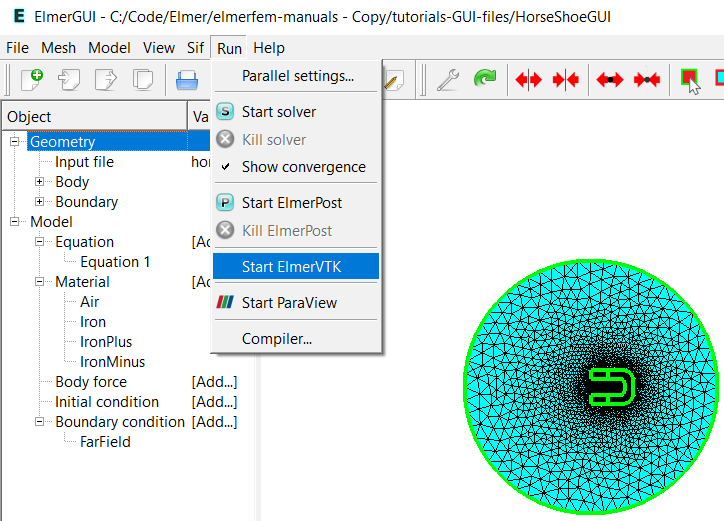
\includegraphics[width=0.8\textwidth]{vtk-1}
\caption{Start ElmerVTK}\label{fg:vtk-1}
\end{center}
\end{figure}

The ElmerVTK window will open, displaying the geometry,  as shown in Figure~\ref{fg:vtk-2}.  Click on the menu bar for the `Isocontours' menu.  In two places, variable and color, click for the drop down menu and select `potential'.

\begin{figure}[H]
\begin{center}
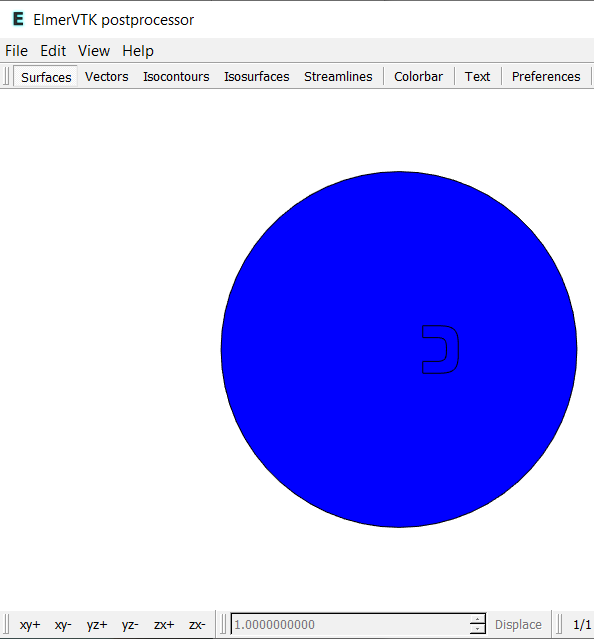
\includegraphics[width=0.45\textwidth]{vtk-2}
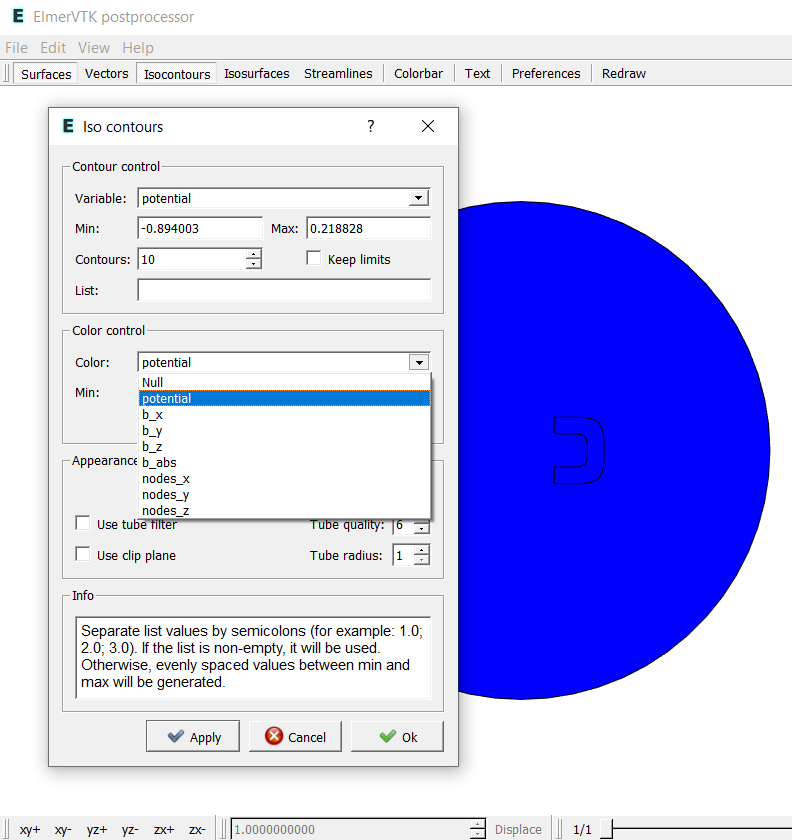
\includegraphics[width=0.45\textwidth]{vtk-3}
\caption{ElmerVTK showing geometry, select Isocontours}\label{fg:vtk-2}
\end{center}
\end{figure}

The isocontours of potential will show, superimposed on the geometry, as shown in Figure~\ref{fg:vtk-4}.  The number of isocontours look a little sparse, so open up the Isocontours menu again, and this time change number of `Contours' from 10 to 50.  That looks better.

\begin{figure}[H]
\begin{center}
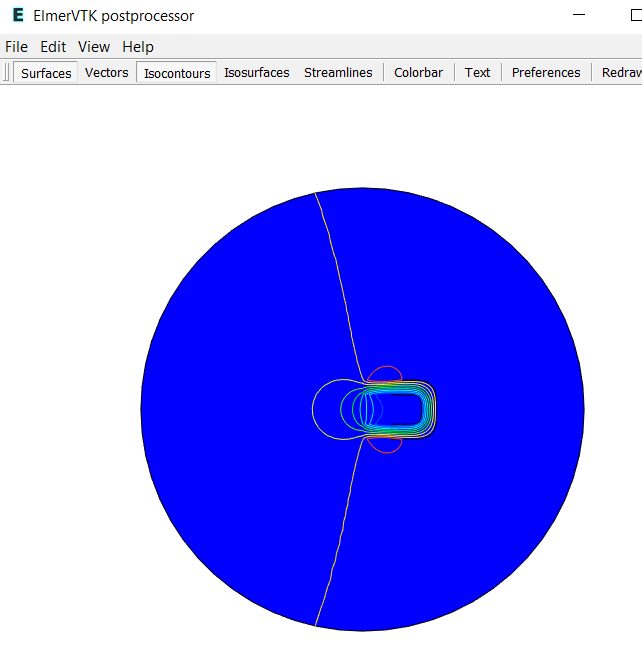
\includegraphics[width=0.48\textwidth]{vtk-4}
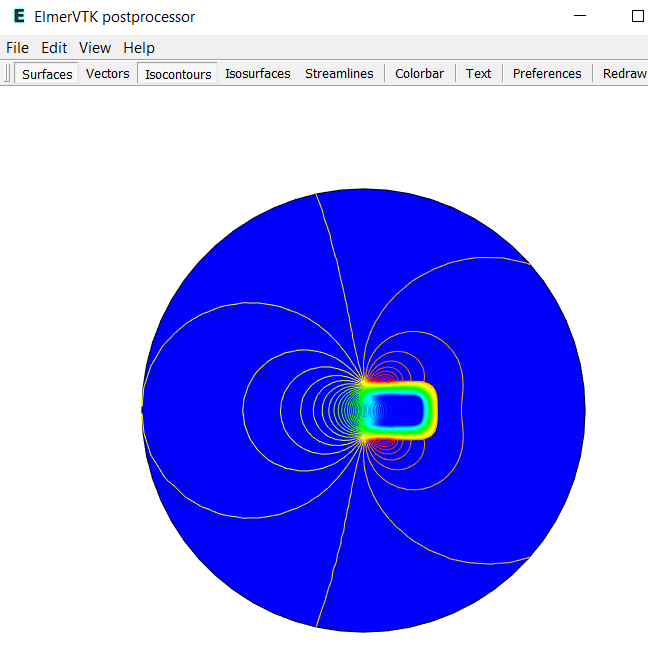
\includegraphics[width=0.48\textwidth]{vtk-5}
\caption{Isocontours of potential, 10 on left, 50 on right}\label{fg:vtk-4}
\end{center}
\end{figure}

\newpage

Next, let's add a color bar, as shown in Figure~\ref{fg:vtk-4}, so we can see the range of values shown on the plot.

\begin{figure}[H]
\begin{center}
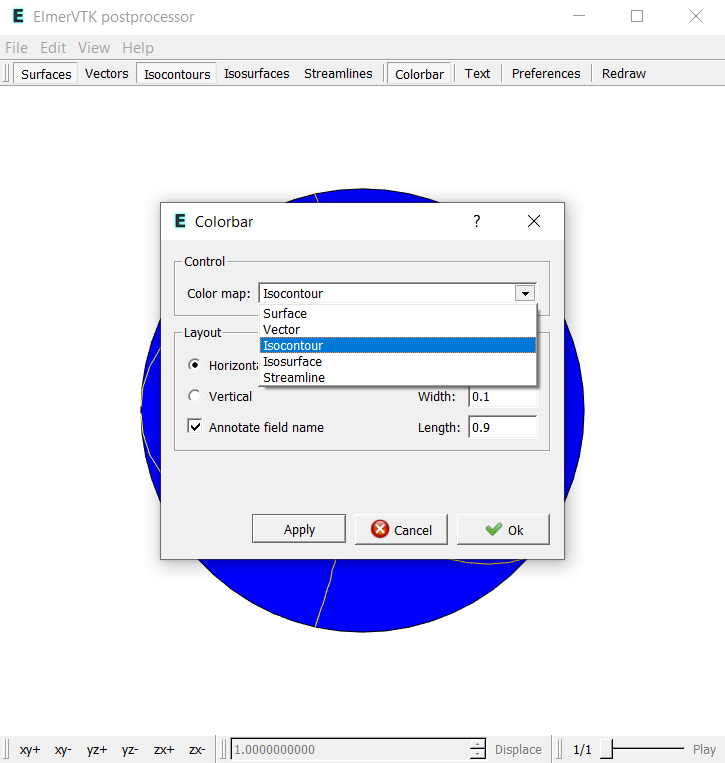
\includegraphics[width=0.48\textwidth]{vtk-6}
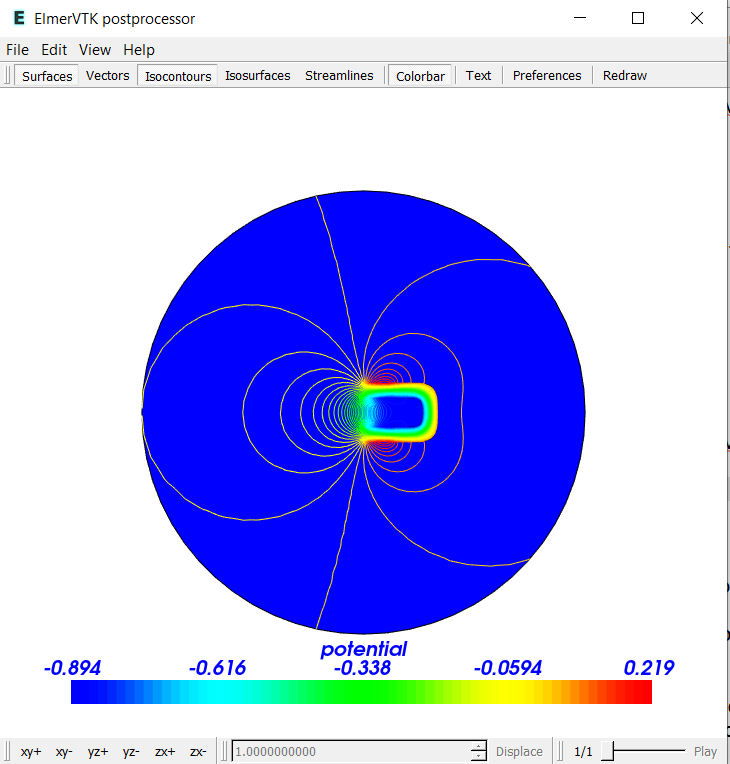
\includegraphics[width=0.48\textwidth]{vtk-7}
\caption{Add a Color Bar}\label{fg:vtk-6}
\end{center}
\end{figure}

We used a 2D example, so the choice of Isocontours made sense.  If we had used a 3D example, like the first heat tutorial, then Isosurfaces would make more sense.\\

As promised, ElmerVTK is fairly simple to use, and will make some pretty nice graphics in a short amount of time.

%%%%%%%%%%%%%%%%%%%%%%%%%%%%

\chapter{More Information -- Elmer -- Windows}

\section{Windows -- Open a Command Prompt Anywhere}

Most Windows programs use the graphical interface and so most Windows users have little experience using the command prompt.  Being proficient with the command prompt is useful when working with Elmer, such as running Elmergrid or running Elmersolver.\\

Windows includes the command prompt window and also Powershell, which is a more recent version.  For our purposes, either one is sufficient, and these notes will apply to both.\\

First, one can open a command window by clicking on the Start button, and then just start typing `command', and select the bar for `Command Prompt'.  Likewise, click on the start button and start typing `powershell', and select the bar for `PowerShell'.  From here on to make things simpler, we will only use `Command Prompt' for these examples.\\

The Command Prompt window will open, and the default directory (C:/Users/...>) will be shown with a blinking cursor.  Since the default directory is almost never the directory you want, there must be a better method of opening a command prompt window.\\

Windows includes File Explorer, which most people use all the time to navigate directories and files within Windows.  One way to open File Explorer is to click on the start button, and start typing `file explorer' and select the bar for `File Explorer'.  You may already have shortcuts to open File Explorer on your desktop or on the taskbar, so use whatever method you prefer to open File Explorer.\\

Let's assume that you have already created \texttt{C:/Elmer/PassiveElements}, by copying one of the tutorials.  Open File Explorer and navigate to the PassiveElements folder.  You will see the folder with the directory contents on the right, and there will be a bar near the top containing: \texttt{This PC > Local Disk (C:) > Elmer > PassiveElements}.

\begin{figure}[H]
\centering
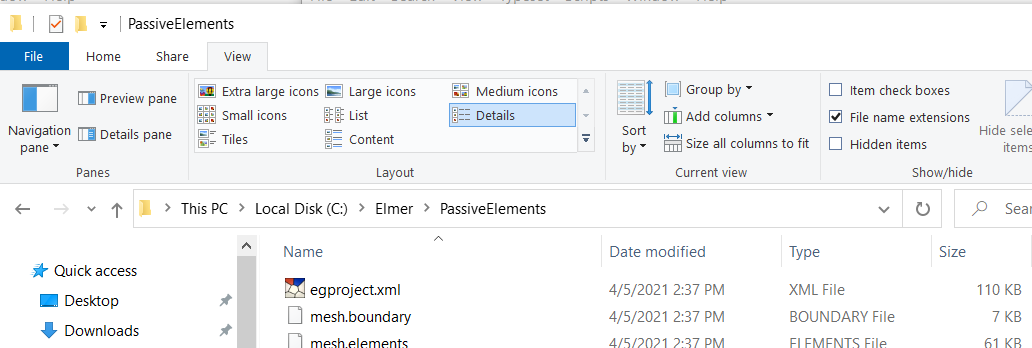
\includegraphics[width=0.7\textwidth]{cmd-1}
\caption{File Explorer}\label{fg:cmd-1}
\end{figure}

Click in the bar with the mouse, and the contents will change to: \texttt{C:/Elmer/PassiveElements}, and will be highlighted in blue.  

\begin{figure}[H]
\centering
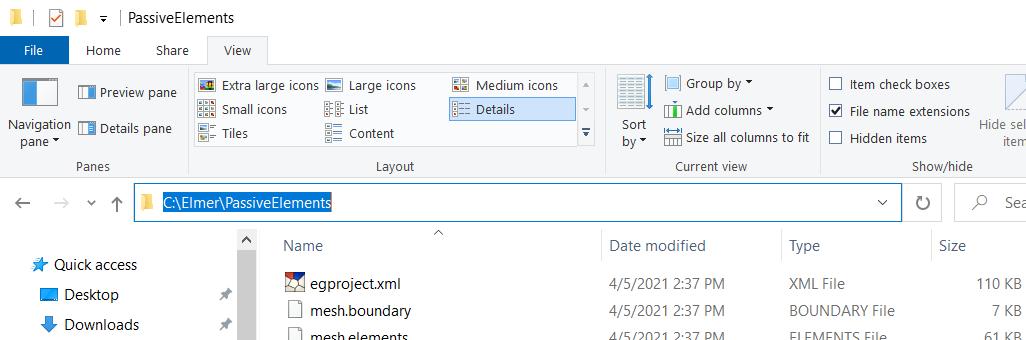
\includegraphics[width=0.9\textwidth]{cmd-2}
\caption{Highlight in Blue}\label{fg:cmd-2}
\end{figure}

While the content is highlighted blue, type `cmd' and press enter.

\begin{figure}[H]
\centering
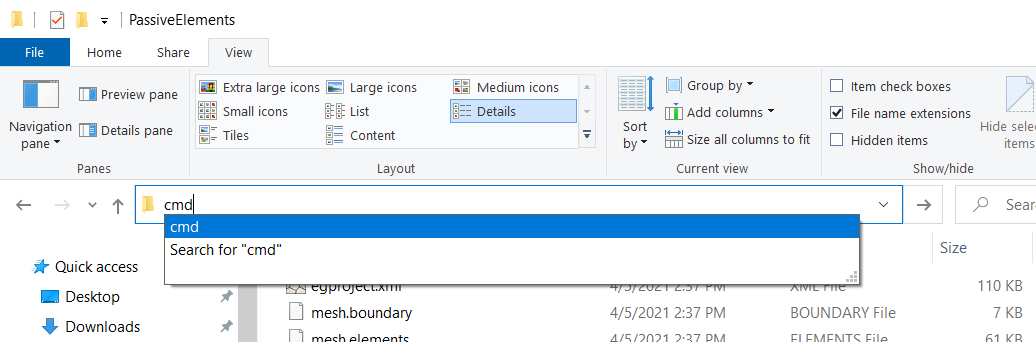
\includegraphics[width=0.9\textwidth]{cmd-3}
\caption{Type in cmd}\label{fg:cmd-3}
\end{figure}

A command prompt window will open up, and will be located in the PassiveElements folder.\\

\begin{figure}[H]
\centering
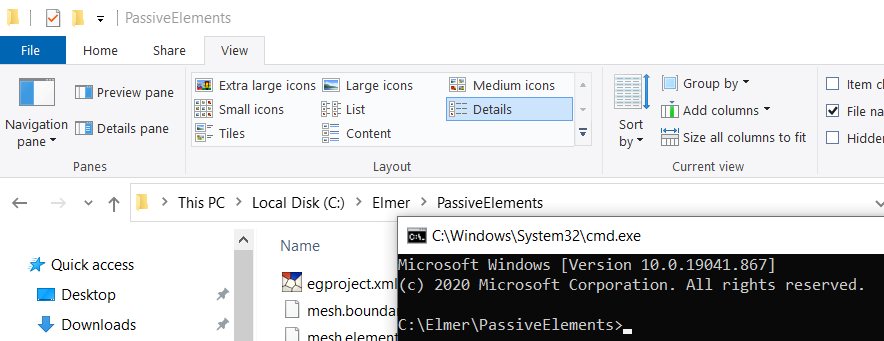
\includegraphics[width=0.9\textwidth]{cmd-4}
\caption{Command prompt window}\label{fg:cmd-4}
\end{figure}

\newpage

One can use the same method to open a Powershell window.  While the content is highlighted blue, type `powershell' and press enter.

\begin{figure}[H]
\centering
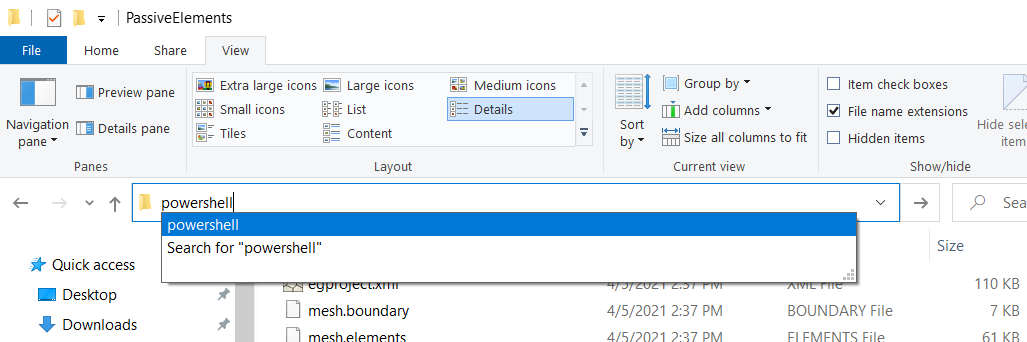
\includegraphics[width=0.9\textwidth]{cmd-5}
\caption{Type in powershell}\label{fg:cmd-5}
\end{figure}

A Powershell window will open up, and will be located in the PassiveElements folder.\\

\begin{figure}[H]
\centering
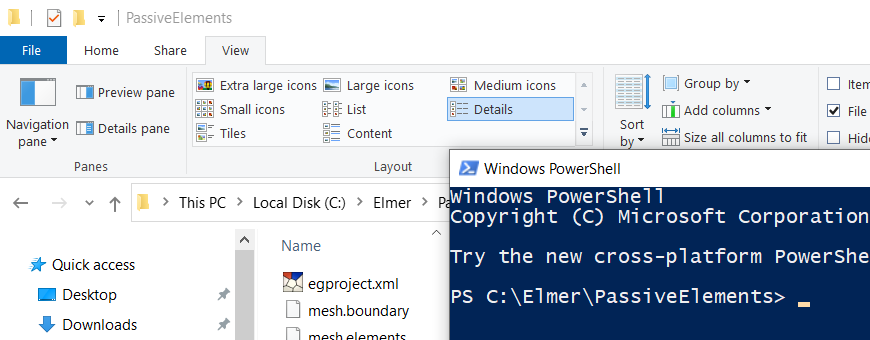
\includegraphics[width=0.9\textwidth]{cmd-6}
\caption{Powershell window}\label{fg:cmd-6}
\end{figure}


The command prompt accepts many commands, such as type `dir', press enter, and a directory listing will appear with the files inside the current folder.  Changing directories is done with the `cd' command.   Type `cd ..' to change to the parent directory, and type `cd PassiveElements' to change back to the sub folder.  If you use the File Explorer and cmd approach to open your command prompt windows, you won't need to use `cd' much.

\section{Windows -- Batch files}

A typical use of the command prompt in Elmer will be to run Elmergrid and Elmersolver.  One can also use batch files to run Elmergrid and Elmersolver, which can be handy and sometimes faster.  For example, use a text editor such as Notepad to create a text file named \texttt{run.bat} with the following contents:

\ttbegin
elmergrid 1 2 mesh
pause
elmersolver
pause
\ttend

This assumes you have a valid elmergrid geometry input file named \texttt{mesh.grd}, an elmer sif file named \texttt{case.sif}, and a file named \texttt{ELMERSOLVER\_STARTINFO} in the same folder as the batch file.  In File Explorer, double click on the file \texttt{run.bat} and a command window will open and Elmergrid will execute, followed by a pause.  Press any key, and elmersolver will execute, followed by a pause.  You have run an Elmer case inside a command window, but without having to actually open a command window or type any commands in the window.  If you are running the same example over and over, and making changes to the sif file each time, then using a batch file will save some time.

\section{Tutorial files}

The Elmer Documentation that was previously downloaded includes working examples of the tutorials, in the folders named  \texttt{tutorials-GUI-files} and  \texttt{tutorials-CL-files}.  These folders include the geometry input files and the egproject files.

\section{Elmerfem test files}

The source code for Elmer is located on github, at \url{https://github.com/ElmerCSC/elmerfem}.  Open that webpage, click on the green button that says \texttt{Code}, and select \texttt{Download ZIP}.  The zip file will download, copy the file to a good folder, such as \texttt{C:/Elmer} and extract the contents.  A new folder named \texttt{elmerfem} will contain the source code for the Elmer suite.  Open the sub folder \texttt{elmerfem/fem/tests} and you will see about 700 folders, one for each test case.  Each test folder will have all the files needed to run each test.  Searching through the 700 folders for a particular solver will lead one to the desired tests.

\section{ElmerGrid sample files}

If you download the github repository as described above in the Elmerfem test files section, there is a folder \texttt{elmerfem/ElmerGUI/samples/grd} that contains samples of elmergrid input files.  These samples plus the ElmerGrid manual will help get started with ElmerGrid.

\section{Elmer Forum}

The Elmer user forum has many years of history, from many users.\\

\url{http://www.elmerfem.org/forum/}\\

There are quite a few example cases contributed by users, and are described nicely in the sub-forum, `Contributed Cases'.

\section{Elmer on Youtube}

There are many videos on Youtube about Elmer, here's a link:\\

\url{https://www.youtube.com/user/elmerfem/videos}

%%%%%%%%%%%%%%%%%%%%%%%%%%%%

\chapter{Elmer and Parallel Solutions}

Running Elmer solutions in parallel is not difficult, whether run from a command prompt or from within ElmerGUI.  As always, make sure you have a project that runs to completion in serial, with a single processor, then you can convert to a parallel run.

\section{Test serial operation}

Let's run an example in serial operation, to make sure we have a working example.  We will also compare the example directory contents between serial and parallel operation, so running the serial example first will be helpful.

Start by creating a new folder that we will use to hold several example directories.  We will use \texttt{C:\textbackslash{}Elmer}, but you can use whatever folder make sense.

Next, let's select an example tutorial to work with, such as \texttt{FlowStepGUI}, and copy the tutorial folder from \texttt{tutorials-GUI-files} into our new folder.

Then copy the newly copied tutorial folder and paste it twice into our new folder, so you end up with three identical folders as shown in Figure~\ref{fg:folders}.

\begin{figure}[H]
\centering
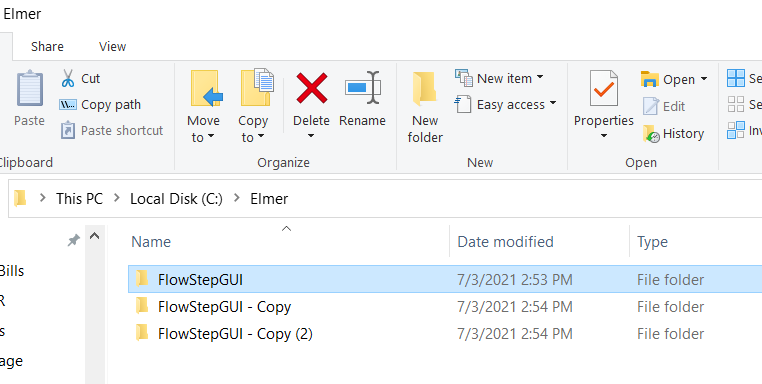
\includegraphics[width=0.8\textwidth]{serial-10}
\caption{Setup example folders}\label{fg:folders}
\end{figure}

\newpage

Let's rename two of the three folders, so we can keep track of our work.  Add a suffix of `serial' and of `parallel', as shown in Figure~\ref{fg:folders-rename}.  Don't rename the folder ending in `- Copy', we'll need it later on.

\begin{figure}[H]
\centering
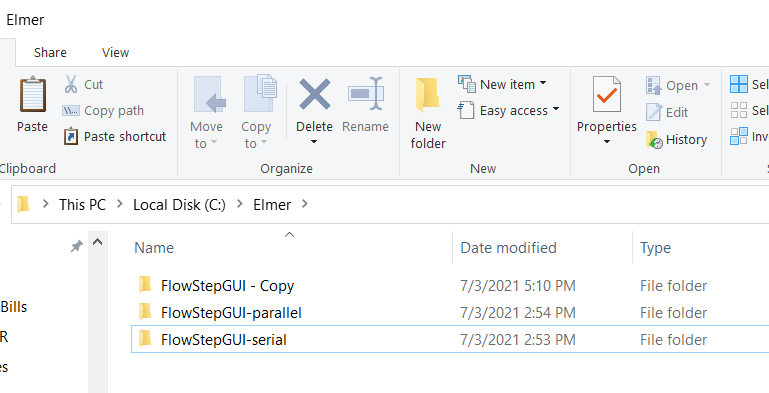
\includegraphics[width=0.8\textwidth]{serial-11}
\caption{Rename two of the example folders}\label{fg:folders-rename}
\end{figure}

Open the folder \texttt{FlowStepGUI-serial} containing the Flow Step tutorial, there will be 6 files as shown in Figure~\ref{fg:folders-orig}.

\begin{figure}[H]
\centering
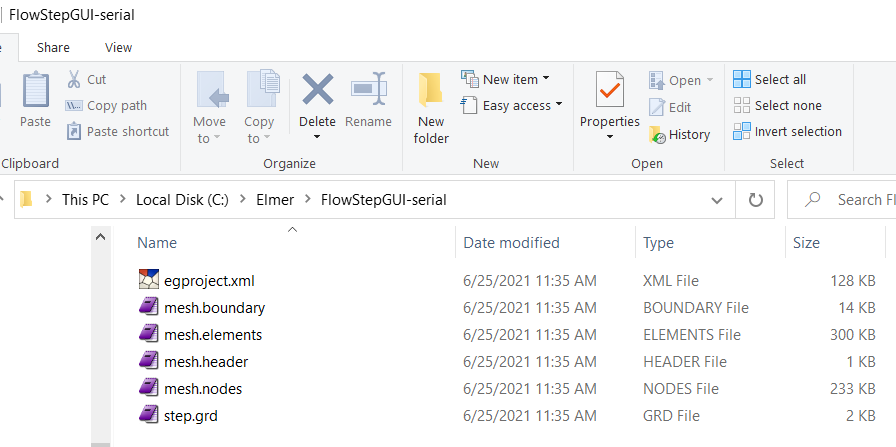
\includegraphics[width=0.8\textwidth]{serial-12}
\caption{Tutorial files}\label{fg:folders-orig}
\end{figure}

\newpage

Start ElmerGUI and \texttt{Load Project} from the folder \texttt{FlowStepGUI-serial}.  Once the project has loaded, click on Run, Parallel Settings, you should see the settings window as shown in Figure~\ref{fg:settings}.  Verify that the box \texttt{Use parallel solver} IS NOT checked.  Click on the \texttt{Accept} button at the bottom of the window.

\begin{figure}[H]
\centering
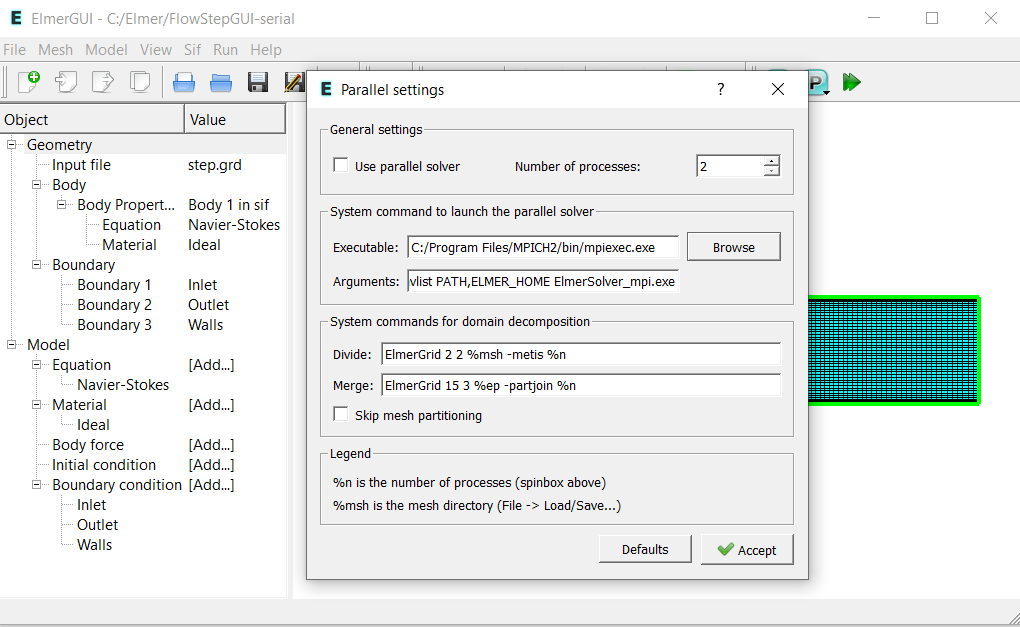
\includegraphics[width=0.8\textwidth]{serial-13}
\caption{Run, Parallel Settings}\label{fg:settings}
\end{figure}

Click on the right green arrow to `Generate and save sif, save project,  then run the solver'.  The solver log window and the convergence history window should pop up and the solver will finish in 4 or 5 seconds.  Refer to Figure~\ref{fg:solver}.

\begin{figure}[H]
\centering
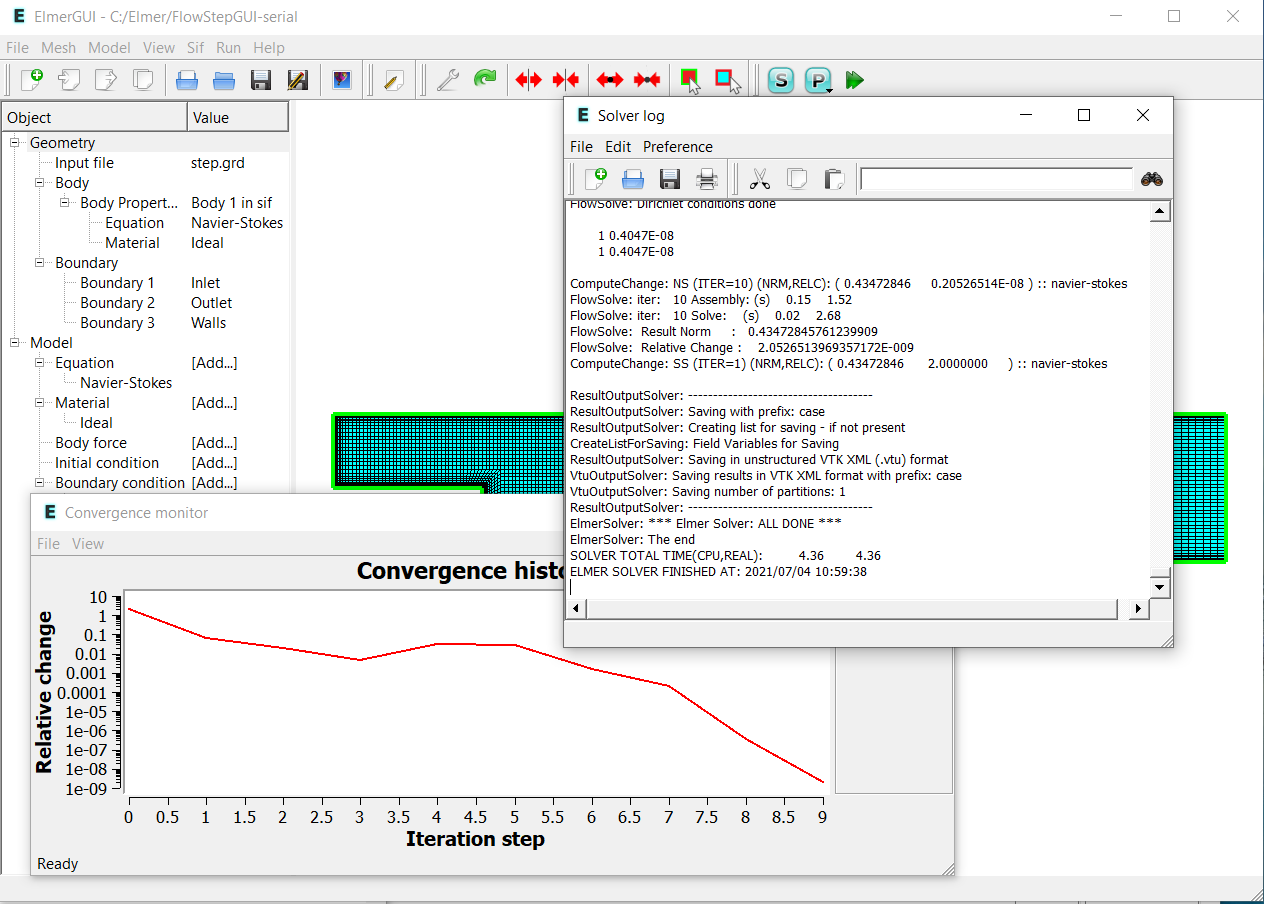
\includegraphics[width=0.8\textwidth]{serial-14}
\caption{Solver Log and Convergence History}\label{fg:solver}
\end{figure}

\newpage

Take a look at the folder \texttt{FlowStepGUI-serial}, now there will be 9 or 10 files, as shown in Figure~\ref{fg:results}.  The file `case.sif' was generated by ElmerGUI and the file `case\_t0001.vtu' is the Paraview results file.

\begin{figure}[H]
\centering
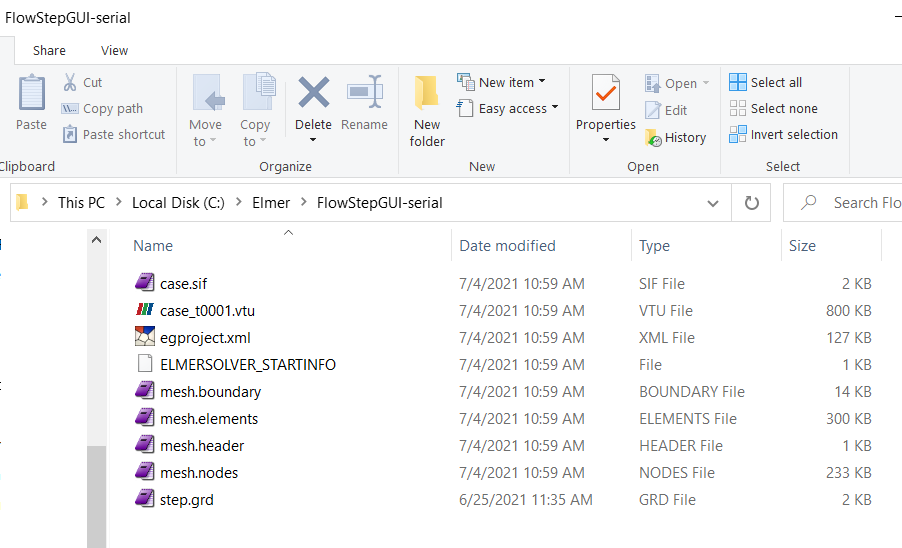
\includegraphics[width=0.8\textwidth]{serial-15}
\caption{Sif and Vtu files}\label{fg:results}
\end{figure}

\section{Parallel settings in ElmerGUI}

We are almost ready to run our example in parallel, but first we must verify the required settings.  The default settings for parallel operation may not work, so we may need to adjust the settings before beginning parallel solutions.  ElmerGUI will store the settings so we only need to go through this step once.  Of course, if a new version of ElmerGUI is installed, then we will need to verify the settings again.  Typical settings for ElmerGUI in Windows 10 are shown in Figure~\ref{fg:parallel-settings}.\\

To activate parallel solutions, check the check box for \texttt{Use parallel solver}.  To change back to serial solution, uncheck this box.  Second, adjust the \texttt{Number of processes} to match the number of physical processors in your system.

Third, enter the name of the executable for MPI.  For Windows, the Elmer Installer will install Microsoft MPI the first time the installer is run, and the name of the executable is \texttt{mpiexec}.  The Microsoft MPI installer will add  \texttt{C:\textbackslash{}Program Files\textbackslash{}Microsoft MPI\textbackslash{}Bin\textbackslash{}mpiexec.exe} to the system Path, so you should not need to add the directory path to the executable, so just enter \texttt{mpiexec}.

When using Linux (such as in the Elmer Virtual Machine), the MPI executable is named \texttt{mpirun}, so one would add \texttt{mpirun} into the Executable box.

Fourth, enter the following into the Arguments box: \texttt{-n \%{}n ElmerSolver\_{}mpi.exe}.  
\texttt{}
The `-n' indicates that the number of processes will be next, followed by `\%{}n' which is a variable placeholder equal to the number of processes selected in the second step above.

Fifth, enter the following into the Divide box: \texttt{ElmerGrid 2 2 \%msh -partdual -metiskway \%n}.  This command calls ElmerGrid with formats 2 and 2, meaning input an Elmer mesh.* and output an Elmer mesh.*.  The \%msh is a variable placeholder equal to the Mesh name.  The commands -partdual and -metiskway are commands used by ElmerGrid when calling Metis to perform the partitioning of the mesh.  Finally, the \%n is a variable placeholder equal to the number of processes selected in the second step above.

The Merge box is not needed because Paraview takes care of merging the resulting .vtu files when displaying the results.

Click on the \texttt{Accept} button at the bottom to save your settings and close the window.

\begin{figure}[H]
\centering
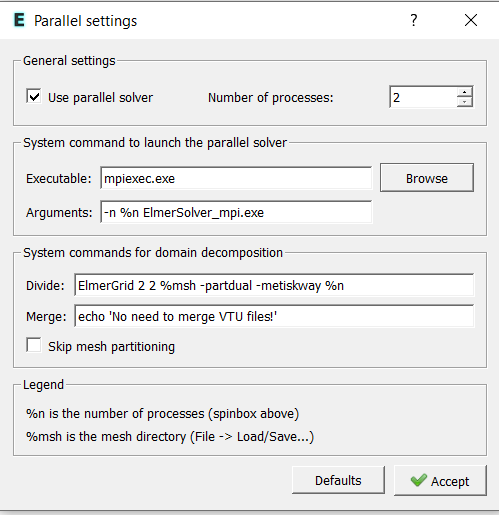
\includegraphics[width=0.8\textwidth]{parallel-settings}
\caption{Parallel settings in ElmerGUI}\label{fg:parallel-settings}
\end{figure}

\section{Test parallel operation}

Start ElmerGUI and \texttt{Load Project} from the folder \texttt{FlowStepGUI-parallel}.  Once the project has loaded, click on Run, Parallel Settings, you should see the settings window as shown in Figure~\ref{fg:parallel-settings}.  Verify that the box \texttt{Use parallel solver} IS checked.  Click on the \texttt{Accept} button at the bottom of the window.

Click on the right green arrow to `Generate and save sif, save project,  then run the solver'.  The solver log window and the convergence history window should pop up and the solver will finish in 2 or 3 seconds.  Refer to Figure~\ref{fg:solver-parallel}.

Take a look at the folder \texttt{FlowStepGUI-parallel}, now there will be 14 or 15 files, as shown in Figure~\ref{fg:results-parallel}.  The file `case.sif' was generated by ElmerGUI and the four files like `case\_4np1\_t0001.vtu' are the Paraview results file for each of the four partitions.  The file `case\_t0001.pvtu' is new, and is the Paraview result file that will merge the four partitions back into a single model.  There is also a new sub-folder `partitioning.4' that contains the partitioned mesh files generated by the call to ElmerGrid.

Well, that was easy.  Now that ElmerGUI has stored the parallel settings in the xml file for this project, all you have to do is check or uncheck the box for \texttt{Use parallel solver} and you can switch from serial to parallel and back to serial operation. 

\begin{figure}[H]
\centering
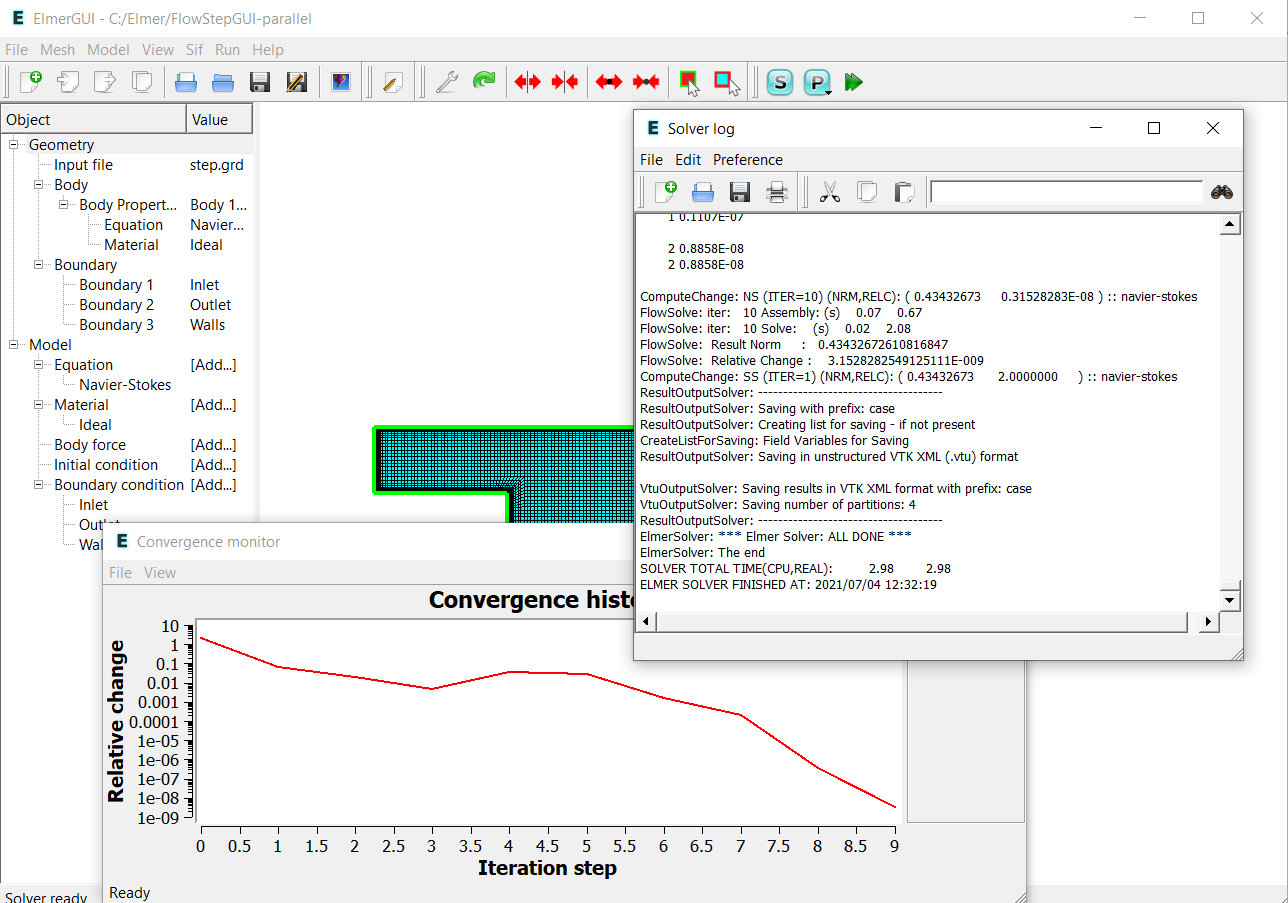
\includegraphics[width=0.85\textwidth]{parallel-10}
\caption{Solver Log and Convergence History}\label{fg:solver-parallel}
\end{figure}

\begin{figure}[H]
\centering
\includegraphics[width=0.85\textwidth]{parallel-11}
\caption{Sif and Vtu files}\label{fg:results-parallel}
\end{figure}

\section{Spaces in path to project}

With verified settings and example tutorial files for practice, what could possibly go wrong?  Let's check to see what happens if there are spaces in the path to your ElmerGUI folder.

Start ElmerGUI and \texttt{Load Project} from the folder \texttt{FlowStepGUI - Copy} that we created before starting `Test serial operation'.  Note that there are two spaces in the directory name.  Once the project has loaded, click on Run, Parallel Settings, you should see the settings window as shown in Figure~\ref{fg:parallel-settings}.  Update the parallel settings, as needed.  Verify that the box \texttt{Use parallel solver} IS checked.  Click on the \texttt{Accept} button at the bottom of the window.

Click on the right green arrow to `Generate and save sif, save project,  then run the solver'.  The solver log window  should pop up and the solver will stop early with errors, as shown in to Figure~\ref{fg:spaces}. 

\begin{figure}[H]
\centering
\includegraphics[width=0.8\textwidth]{parallel-12}
\caption{Spaces in the directory name}\label{fg:spaces}
\end{figure}

 The key error message is `WARNING:: LoadMesh: Requested mesh > ./. < in partition 4 does not exist!'.  Remove the spaces from the directory name, and the errors will go away.  The problem is that the call to ElmerGrid uses the path to the folder, up to the first space.  If you look at the example folders, you will see there are now four folders, and the fourth folder will contain the partitioned mesh files.


\section{Information about Parallel}

For an overview and background information about Elmer parallel operation, download the file \texttt{ElmerParallel.pdf} from this site:\\

\url{http://www.nic.funet.fi/pub/sci/physics/elmer/slides/}


\section{Sif file}

Note that when going from serial to parallel, in general the sif file does not change and only how the project is started changes.  One section in the sif that may change may be the mesh directory, depending on how ElmerGrid is run.  The solver, equation, materials, boundary conditions, etc., should not need any changes.

%%%%%%%%%%%%%%%%%%%%%%%%%%%%

\chapter{Elmer and External Tools}

\section{Multiple bodies from Salome to Elmer}

\subsection{Introduction}

The desired final result of this exercise will be a single Elmer mesh with 3 bodies and 16 boundaries.  The boundaries will be defined for each exterior face of the bodies and the interior faces between each body.  The bodies will allow assignment of two or three materials, with a boundary between each material.\\

The original wiki page described how to create a mesh that contains multiple bodies with Salome MECA 2009 and how to import it in Elmer.  There is a video on Youtube from 2015 based on the elmerfem wiki:\\

\url{https://www.youtube.com/watch?v=xfMLtywHSr4}\\

\noindent This section in Get Started with Elmer has been rewritten in 2021 with new graphics using Salome 9.7.0 and Elmer 9.0.

\subsection{Install Salome}

Download the latest version of Salome from\\

\url{https://www.salome-platform.org/}\\

and follow the instructions to install Salome.  The Salome website has lot's of information, such as user tutorials at:\\

\noindent \url{https://www.salome-platform.org/user-section/salome-tutorials/salome-tutorial}\\

The tutorials will be very helpful for first time users of Salome.  The first tutorial shows the basics of creating geometry, partitioning, and meshing.  After installing and starting Salome, follow these instructions.  Note that we assume you know the basics of Salome, and so we will give high level instructions.

\subsection{Define your geometry in Salome}

First, we need to define a geometry, so activate the Geometry module, as shown in Figure~\ref{fg:salome-01}. 

\begin{figure}[H]
\centering
\includegraphics[width=0.9\textwidth]{Salome-01}
\caption{Geometry module}\label{fg:salome-01}
\end{figure}

In this example we deal with a simple case, with three boxes. We create two boxes which are intersecting each other, using New Entity -> Primitives -> Box, as shown in Figure~\ref{fg:salome-02}.

\begin{figure}[H]
\centering
\includegraphics[width=0.9\textwidth]{Salome-02}
\caption{Box primitive}\label{fg:salome-02}
\end{figure}

Create Box\_1 using the default size at the origin, and increase Dx to 300, as shown in Figure~\ref{fg:salome-03}.

\begin{figure}[H]
\centering
\includegraphics[width=0.9\textwidth]{Salome-03}
\caption{Create Box\_1}\label{fg:salome-03}
\end{figure}

Create Box\_2 using the default size at the origin, and increase Dy to 300, as shown in Figure~\ref{fg:salome-04}.

\begin{figure}[H]
\centering
\includegraphics[width=0.9\textwidth]{Salome-04}
\caption{Create Box\_2}\label{fg:salome-04}
\end{figure}

Use Operations -> Boolean -> Cut, as shown in Figure~\ref{fg:salome-05}.

\begin{figure}[H]
\centering
\includegraphics[width=0.9\textwidth]{Salome-05}
\caption{Boolean Cut}\label{fg:salome-05}
\end{figure}

Cut Box\_2 using Box\_1 as the tool, which will create the third box, as shown in Figure~\ref{fg:salome-06}.  Of course, you could as well define three separate boxes that share their respective surfaces geometrically. In this example, let's stick with the two intersecting boxes.

\begin{figure}[H]
\centering
\includegraphics[width=0.9\textwidth]{Salome-06}
\caption{Create Cut\_1}\label{fg:salome-06}
\end{figure}

We now have three boxes, named Box\_1, Box\_2, and Cut\_1, as shown in Figure~\ref{fg:salome-07}.  Note the small icon shown just above the little tool tip `Global Panning', which expanded the object to fill the view port.  Also, note that we can check the shape of each box using the visibility icon, the little eye just to the left of the entity in the geometry tree.

\begin{figure}[H]
\centering
\includegraphics[width=0.9\textwidth]{Salome-07}
\caption{Three boxes}\label{fg:salome-07}
\end{figure}

Next, let's cut again to make another small box, this time using Box\_2 to cut Box\_1, as shown in Figure~\ref{fg:salome-08}.  It may seem that some of the boxes disappear after performing the cut, but they are just invisible, so use the eye icon to make them reappear.

\begin{figure}[H]
\centering
\includegraphics[width=0.9\textwidth]{Salome-08}
\caption{Create Cut\_2}\label{fg:salome-08}
\end{figure}

For the last step, select the Operation, Boolean, Common, menu item, as shown in Figure~\ref{fg:salome-09}.

\begin{figure}[H]
\centering
\includegraphics[width=0.9\textwidth]{Salome-09}
\caption{Common menu}\label{fg:salome-09}
\end{figure}

This step will create Common\_1, a cube, as shown in Figure~\ref{fg:salome-10}.

\begin{figure}[H]
\centering
\includegraphics[width=0.9\textwidth]{Salome-10}
\caption{Create Common\_1}\label{fg:salome-10}
\end{figure}

We have successfully created three solid objects.  The objects share common nodes at the edges of each object and the volumes of each object do not overlap.

\subsection{Partition the geometry}

Now we have defined our geometry, but it is not yet ready for meshing. Because Elmer expects a single mesh, you need a single `object' for the meshing operation and now you have three objects. Therefore we need to combine these three solid objects together, before starting the meshing operation.

IT WOULD be natural to create a compound object which contains three solids, but this is not right way to do it. Because, when you create a compound, Salome will consider the solids as individuals and creates three separate meshes that when exported to unv will create three separate mesh files.  When you try to load each mesh in ElmerGUI, you will have three separate models, which can't be combined into one Elmer solution.

What we need to do is to use the Salome operation called, Partition.  Using an analogy from computer file systems, one can create a partition to hold multiple disk drives, so in a similar fashion in Salome we will create a partition to hold several CAD objects as solid objects.

First, let's select three items in the geometry tree, Cut\_1, Cut\_2, and Common\_1.  Then use menu selection Operations -> Partition, as shown in Figure~\ref{fg:salome-11}.

\begin{figure}[H]
\centering
\includegraphics[width=0.9\textwidth]{Salome-11}
\caption{Partition menu}\label{fg:salome-11}
\end{figure}

We will create Partition\_1 from 3 objects, as shown in Figure~\ref{fg:salome-12}.

\begin{figure}[H]
\centering
\includegraphics[width=0.9\textwidth]{Salome-12}
\caption{Create Partition}\label{fg:salome-12}
\end{figure}

Partition\_1 now shows up with three sub-objects, as shown in Figure~\ref{fg:salome-13}.  

\begin{figure}[H]
\centering
\includegraphics[width=0.9\textwidth]{Salome-13}
\caption{Partition\_1}\label{fg:salome-13}
\end{figure}

We have one more step before we can start meshing the geometry.  We need to be able to select bodies within the partition, so we must use the menu selection New Entity -> Explode, as shown in Figure~\ref{fg:salome-14}.

\begin{figure}[H]
\centering
\includegraphics[width=0.9\textwidth]{Salome-14}
\caption{Explode menu}\label{fg:salome-14}
\end{figure}

Be sure to select `Sub-shapes Type' as `solid', as shown in Figure~\ref{fg:salome-15}.

\begin{figure}[H]
\centering
\includegraphics[width=0.9\textwidth]{Salome-15}
\caption{Select solid type}\label{fg:salome-15}
\end{figure}

Expanding Partition\_1 in the geometry tree shows three solids are now available, as shown in Figure~\ref{fg:salome-16}.

\begin{figure}[H]
\centering
\includegraphics[width=0.9\textwidth]{Salome-16}
\caption{Three solids}\label{fg:salome-16}
\end{figure}

\subsection{Create the mesh}

At this point you can move to the mesh module, to create a mesh for the partition object.  In this example we use automatic netgen 1D-2D-3D as the mesh generator.  Select the Mesh module instead of the Geometry module from the menu, as shown in Figure~\ref{fg:salome-17}.  You may need to once again use the eye icons to make the objects visible.

\begin{figure}[H]
\centering
\includegraphics[width=0.9\textwidth]{Salome-17}
\caption{Mesh module}\label{fg:salome-17}
\end{figure}

Next, make sure that Partition\_1 is highlighted in the tree, then select Mesh -> Create Mesh menu option, as shown in Figure~\ref{fg:salome-18}.

\begin{figure}[H]
\centering
\includegraphics[width=0.9\textwidth]{Salome-18}
\caption{Create Mesh}\label{fg:salome-18}
\end{figure}

In the Algorithm box, select NETGEN 1D-2D-3D, as shown in Figure~\ref{fg:salome-19}.

\begin{figure}[H]
\centering
\includegraphics[width=0.9\textwidth]{Salome-19}
\caption{NETGEN 1D-2D-3D}\label{fg:salome-19}
\end{figure}

\subsection{Refine the mesh}

We could accept the default mesh settings and proceed to computing the mesh, but that isn't a typical usage.  Let's use Netgen to refine the mesh while computing the mesh.  Click on the settings box to the right of the Hypothesis box, and select NETGEN 3D Parameters, as shown in Figure~\ref{fg:salome-20}.

\begin{figure}[H]
\centering
\includegraphics[width=0.9\textwidth]{Salome-20}
\caption{Netgen Parameters}\label{fg:salome-20}
\end{figure}

Change Max size to 20 and Min size to 10, as shown in Figure~\ref{fg:salome-21}.  Netgen will use these parameters to decide on element sizes.  Notice that Netgen is also capable of generating second order elements (in 2D and 3D) and quad dominated elements (in 2D only), just by checking the appropriate boxes in this window.\\

When using an Elmer solver for elasticity, use of second order elements is recommended.  When using an Elmer solver for Navier-Stokes flow, some experts recommend using second order elements.\\

As a side note, you can create a first mesh using first order elements, and then create a second mesh using second order elements, and export each mesh into two separate UNV files.  Then use the UNV files to compare the effect of first order versus second order elements in Elmer.

\begin{figure}[H]
\centering
\includegraphics[width=0.9\textwidth]{Salome-21}
\caption{Max and Min element sizes}\label{fg:salome-21}
\end{figure}

\subsection{Compute the mesh}

That finishes definition of our desired mesh, next step is to tell Salome to actually generate the mesh, by selecting Mesh -> Compute, as shown in Figure~\ref{fg:salome-22}.

\begin{figure}[H]
\centering
\includegraphics[width=0.9\textwidth]{Salome-22}
\caption{Compute the mesh}\label{fg:salome-22}
\end{figure}

A progress window will pop up, as shown in Figure~\ref{fg:salome-23}.

\begin{figure}[H]
\centering
\includegraphics[width=0.9\textwidth]{Salome-23}
\caption{Progress}\label{fg:salome-23}
\end{figure}

The final mesh results summary will then be displayed, as shown in Figure~\ref{fg:salome-24}.

\begin{figure}[H]
\centering
\includegraphics[width=0.9\textwidth]{Salome-24}
\caption{Mesh results}\label{fg:salome-24}
\end{figure}

The computed mesh will be as shown in Figure~\ref{fg:salome-25}.  Notice that under Mesh\_1, there is an entry for `Groups of Volumes', but doesn't show anything for Faces.

\begin{figure}[H]
\centering
\includegraphics[width=0.9\textwidth]{Salome-25}
\caption{Mesh}\label{fg:salome-25}
\end{figure}

\subsection{Create Groups of Faces}

If we exported the mesh at this point, we would have bodies in ElmerGUI, but only one single boundary around the entire body, which is not at all usable.  We need to ask Salome to create faces that will become our individual boundaries.  Select Mesh -> Face groups separated by sharp edges, as shown in Figure~\ref{fg:salome-26}.

\begin{figure}[H]
\centering
\includegraphics[width=0.9\textwidth]{Salome-26}
\caption{Face groups}\label{fg:salome-26}
\end{figure}

Accept the default settings and Apply and Close, as shown in Figure~\ref{fg:salome-27}.

\begin{figure}[H]
\centering
\includegraphics[width=0.9\textwidth]{Salome-27}
\caption{Default face groups}\label{fg:salome-27}
\end{figure}

We now have Groups of Faces under the mesh tree, as shown in Figure~\ref{fg:salome-28}.

\begin{figure}[H]
\centering
\includegraphics[width=0.9\textwidth]{Salome-28}
\caption{Groups of Faces}\label{fg:salome-28}
\end{figure}

\subsection{Export the mesh}

We are now ready to export our mesh, once again make sure to highlight Mesh\_1 in the tree, then select File -> Export -> UNV file, as shown in Figure~\ref{fg:salome-29}.

\begin{figure}[H]
\centering
\includegraphics[width=0.9\textwidth]{Salome-29}
\caption{Export menu}\label{fg:salome-29}
\end{figure}

Save the file, with an appropriate name, in an appropriate directory, as shown in Figure~\ref{fg:salome-30}.  Salome will automatically add the `unv' file extension to the file name.

\begin{figure}[H]
\centering
\includegraphics[width=0.9\textwidth]{Salome-30}
\caption{Save UNV file}\label{fg:salome-30}
\end{figure}

We now have a UNV file containing all the information needed by Elmer to import the example Salome CAD model as three bodies with sixteen boundaries and with a refined tetrahedral mesh.

\subsection{Summary: Short Version}

The above section shows in great detail how to create a multi-body mesh for Elmer, and it is highly recommended to go through each step the first time to get familiar with the location of each step.  The second or third time going through the steps should be faster and easier, and not as much detail is needed to help create a mesh for Elmer.\\

\noindent Here is a short version of the steps to be taken in Salome to create multiple bodies for export to Elmer.\\

>> Select the Geometry module.\\

>> Create your 3D solid bodies.  They should not overlap their volumes and they should share common nodes.\\

>> Highlight the solid bodies and then `Operations -> Partition'.  Be sure to select Resulting Type as `solid'.\\

>> Highlight the Partition, and then `New Entity -> Explode'.  Be sure to select Sub-shapes Type as `solid'.\\

>> Select the Mesh module.\\

>> Select the Partition and then `Mesh -> Create Mesh'.  In the Algorithm box, select `NETGEN 1D-2D-3D'.  In the Hypothesis box, select `NETGEN 3D Parameters'.  Change Max and/or Min sizes as needed, and select second order as needed.\\

>> Select `Mesh -> Compute Mesh' to generate the mesh.\\

>> Highlight the Mesh and then `Mesh -> Face groups separated by sharp edges', and accept the default settings.\\

>> Highlight the Mesh and then `File -> Export -> UNV file', and save the UNV file with an appropriate name and directory.\\

\noindent This ends the short version.

%%%%%%%%%%%%%%%%%

\newpage

\section{Elmer and UNV files}

The previous section showed how to create and export a UNV file from Salome, ready to be used by Elmer.  This section will show how to use that UNV file in Elmer.\\

For non-GUI users of Elmer, use ElmerGrid in a command prompt or terminal window to convert the UNV file into Elmer mesh format with this command:\\

\texttt{Elmergrid 8 2 mesh\_1 -autoclean}\\

ElmerGUI can read the UNV file directly, and ElmerGUI will then call ElmerGrid in the background to perform the conversion to Elmer mesh format.  This section shows step by step how to read and use the UNV file in ElmerGUI.\\

As a side note, non-GUI users of Elmer may find it useful to use ElmerGUI to perform the conversion from UNV to Elmer mesh format.  ElmerGUI can group boundary faces together, thereby reducing the number of boundary faces into manageable groups.  When ElmerGUI saves the mesh to Elmer mesh format, the reduced number of boundary groups will be written to the files.

\subsection{Open UNV file}

After starting ElmerGUI, select File -> Open, as shown in Figure~\ref{fg:elmergui-1}, then select the Mesh\_1.unv file that you created in the previous section.

\begin{figure}[H]
\centering
\includegraphics[width=0.9\textwidth]{elmergui-1}
\caption{File -> Open}\label{fg:elmergui-1}
\end{figure}

\newpage

ElmerGUI will read the file and based on the file extension, ElmerGUI will automatically call ElmerGrid to perform the conversion, as shown in Figure~\ref{fg:elmergui-2}.

\begin{figure}[H]
\centering
\includegraphics[width=0.9\textwidth]{elmergui-2}
\caption{Imported model}\label{fg:elmergui-2}
\end{figure}

Examine the model parameters by selecting Model -> Summary from the menu, which will open a window to display the various dimensions of the mesh and model, as shown in Figure~\ref{fg:elmergui-3}.

\begin{figure}[H]
\centering
\includegraphics[width=0.9\textwidth]{elmergui-3}
\caption{Model -> Summary}\label{fg:elmergui-3}
\end{figure}

Having a model with sixteen boundaries can be useful, but sometimes we only need a couple of the boundaries.  ElmerGUI can group faces together, which will reduce the number of boundaries, making it easier to manage working with the boundaries.\\

\newpage

Use the mouse and double click on a face to select that face, followed by holding down the ctrl key and double clicking on two more faces, so three faces are highlighted, as shown in Figure~\ref{fg:elmergui-4}.

\begin{figure}[H]
\centering
\includegraphics[width=0.9\textwidth]{elmergui-4}
\caption{Select with ctrl double click}\label{fg:elmergui-4}
\end{figure}

Select Mesh -> Unify surface, as shown in Figure~\ref{fg:elmergui-5}.

\begin{figure}[H]
\centering
\includegraphics[width=0.9\textwidth]{elmergui-5}
\caption{Mesh -> Unify surface}\label{fg:elmergui-5}
\end{figure}

The three faces will be united into one face, so the list of boundaries will decrease from 16 down to 14 boundaries.  

\newpage

Double click on the new unified face, and select View -> Hide/show selected, as shown in Figure~\ref{fg:elmergui-6}.

\begin{figure}[H]
\centering
\includegraphics[width=0.9\textwidth]{elmergui-6}
\caption{Hide/show selected}\label{fg:elmergui-6}
\end{figure}

The selected face will be hidden from view, to reveal the interior boundary faces, as shown in Figure~\ref{fg:elmergui-7}.

\begin{figure}[H]
\centering
\includegraphics[width=0.9\textwidth]{elmergui-7}
\caption{Interior boundaries}\label{fg:elmergui-7}
\end{figure}

This was a brief introduction to importing UNV files into Elmer and ElmerGUI.

%%%%%%%%%%%%%%%%%

\newpage

\section{Elmer and Gmsh}

Gmsh is a `A three-dimensional finite element mesh generator with built-in pre- and post-processing facilities' as described at \url{https://gmsh.info/}\\

Gmsh works well to generate Elmer meshes, and like most three dimensional programs, Gmsh has a  learning curve.  This tutorial is meant to show a complete beginner how to get started with Gmsh, and how to use Gmsh to create meshes for Elmer.\\

The 3D example we will use for this section will follow the example used for the section titled: ` Multiple bodies from Salome to Elmer', where we used two boxes to create three separate volumes, along with 16 separate boundaries.  The three separate volumes will then be meshed, ready to load into ElmerGUI, for use with ElmerSolver.

\subsection{Gmsh basics}

Upon starting Gmsh, it will open a default file named `untitled.geo', as shown in in the title bar in  Figure~\ref{fg:gmsh-01}.

\begin{figure}[H]
\centering
\includegraphics[width=0.9\textwidth]{gmsh-01}
\caption{Startup screen}\label{fg:gmsh-01}
\end{figure}

The first step should be to select \texttt{ File -> New}, as shown in Figure~\ref{fg:gmsh-02}.

\begin{figure}[H]
\centering
\includegraphics[width=0.9\textwidth]{gmsh-02}
\caption{File -> New}\label{fg:gmsh-02}
\end{figure}

Pick your own desired file name and directory and click on \texttt{Save}, as shown in Figure~\ref{fg:gmsh-03}.

\begin{figure}[H]
\centering
\includegraphics[width=0.9\textwidth]{gmsh-03}
\caption{Enter new file name}\label{fg:gmsh-03}
\end{figure}

Gmsh will give you  the option to select your Cad Factory, either OpenCASCADE or Built-in, as shown in Figure~\ref{fg:gmsh-04}, please click on \texttt{OpenCASCADE}.

\begin{figure}[H]
\centering
\includegraphics[width=0.9\textwidth]{gmsh-04}
\caption{Select OpenCASCADE}\label{fg:gmsh-04}
\end{figure}

\newpage

You now have a new file with your desired filename and directory, loaded and active in Gmsh, as shown in Figure~\ref{fg:gmsh-05}.  Notice the bottom bar, which shows `Done reading' with the path to our new file.

\begin{figure}[H]
\centering
\includegraphics[width=0.9\textwidth]{gmsh-05}
\caption{Done reading}\label{fg:gmsh-05}
\end{figure}

Gmsh writes actions to the .geo file as the actions are performed.  The bottom bar says `Done reading', because Gmsh reads the .geo file after writing the .geo file.  Let's open the directory containing the .geo file, as shown in Figure~\ref{fg:gmsh-06}.

\begin{figure}[H]
\centering
\includegraphics[width=0.9\textwidth]{gmsh-06}
\caption{Open directory}\label{fg:gmsh-06}
\end{figure}

Open the .geo file using your favorite text editor, as shown in Figure~\ref{fg:gmsh-07}.  As you can see, Gmsh has written two lines into the .geo file, and shows our selection of OpenCASCADE for the CAD Factory.  We will perform this same action, opening the .geo file using a text editor, at several points in this tutorial, because it is helpful in understanding the actions performed by Gmsh.

\begin{figure}[H]
\centering
\includegraphics[width=0.9\textwidth]{gmsh-07}
\caption{Geo file contents}\label{fg:gmsh-07}
\end{figure}

\subsection{Add Geometry}

Let's add some geometry to our project.  Expand the Geometry menu by clicking on the `plus' sign in front of Geometry.   Likewise, click on the preceding `plus' sign before `Elementary entities', followed by `Add'.  A long list of geometry entities are shown, we are looking for `Box' near the bottom, as shown in Figure~\ref{fg:gmsh-08}.  Go ahead and click on `Box'.

\begin{figure}[H]
\centering
\includegraphics[width=0.9\textwidth]{gmsh-08}
\caption{Add -> Box}\label{fg:gmsh-08}
\end{figure}

The pop up window titled `Elementary Entity Context', will open, as shown in Figure~\ref{fg:gmsh-09}.  Notice that moving the mouse around the viewport will cause the red box to move as well.  Also notice the text instructions in the viewport, in particular, notice `e' to add box and `q' to quit.  Either pressing the `e' key or clicking on `Add', will add a box to the geo file.

\begin{figure}[H]
\centering
\includegraphics[width=0.9\textwidth]{gmsh-09}
\caption{Floating box}\label{fg:gmsh-09}
\end{figure}

We want to force the location of the box to be at the origin.  Click on the three check boxes next to `Freeze', which will freeze the x, y, and z locations from moving with the mouse motion.  Enter 0 into the X, Y, and Z entry boxes, as shown in Figure~\ref{fg:gmsh-10}.  You can see that the lower left corner of the red box is now located at the origin.

\begin{figure}[H]
\centering
\includegraphics[width=0.9\textwidth]{gmsh-10}
\caption{Locate the box at the origin}\label{fg:gmsh-10}
\end{figure}

Let's set the size of the box to be DX = 300, DY = 200, and DZ = 200, by typing the numbers into the entry boxes, followed by clicking on `Add', as shown in Figure~\ref{fg:gmsh-11}.  Elmer uses SI units, (actually Elmer is unit-less, but in practical terms think of SI units as the active units in Elmer) so when running ElmerSolver these dimensions will be in meters.  You can scale the dimensions in Elmer, look up `Coordinate Scaling', which will allow one to easily convert from millimetres to meters.

\begin{figure}[H]
\centering
\includegraphics[width=0.9\textwidth]{gmsh-11}
\caption{Enter box dimensions}\label{fg:gmsh-11}
\end{figure}

\newpage

Let's open up our .geo file in our text editor, to see what Gmsh has done so far, as shown in Figure~\ref{fg:gmsh-12}.  You will see that we have successfully added a box, located at the origin, and with our dimensions.

\begin{figure}[H]
\centering
\includegraphics[width=0.9\textwidth]{gmsh-12}
\caption{Open directory}\label{fg:gmsh-12}
\end{figure}

Notice that the pop up window stayed open after clicking on `Add', waiting for us to either enter more boxes or to press `q' to close the pop up window.  Let's add a second box at the origin, with dimensions of DX = 200, DY = 300, and DZ = 200, and then click on `Add', as shown in Figure~\ref{fg:gmsh-13}.

\begin{figure}[H]
\centering
\includegraphics[width=0.9\textwidth]{gmsh-13}
\caption{Add a second box}\label{fg:gmsh-13}
\end{figure}

Let's open up our .geo file in our text editor, and we see that a second box has been added, as shown in Figure~\ref{fg:gmsh-14}.

\begin{figure}[H]
\centering
\includegraphics[width=0.9\textwidth]{gmsh-14}
\caption{Geo file with two boxes}\label{fg:gmsh-14}
\end{figure}

\subsection{Undo operation}

What if we add another box by accidentally clicking on `Add' too many times?  Let's look at the geo file, as shown in Figure~\ref{fg:gmsh-15}.  We see that now there are three boxes, while we really only want two boxes.  How can we fix this situation?  

\begin{figure}[H]
\centering
\includegraphics[width=0.9\textwidth]{gmsh-15}
\caption{Too many boxes}\label{fg:gmsh-15}
\end{figure}

If we collapse the Elementary Entities menu, as shown in Figure~\ref{fg:gmsh-16}, we will notice the menu item `Remove last script command'.  Click on that menu item, and check the geo file, you will see the third box is now gone.

\begin{figure}[H]
\centering
\includegraphics[width=0.9\textwidth]{gmsh-16}
\caption{Last script command and a Side view}\label{fg:gmsh-16}
\end{figure}

\newpage

\subsection{Viewport and Visibility}

Continuing with our sequence of steps, in the Gmsh viewport we see what could be two boxes, from the side, as shown in the preceding Figure~\ref{fg:gmsh-16}.  In the viewport, click a single left mouse button (LMB) and drag the boxes, and the boxes rotate slightly showing a 3D view of the two boxes, as shown in Figure~\ref{fg:gmsh-17}.

\begin{figure}[H]
\centering
\includegraphics[width=0.9\textwidth]{gmsh-17}
\caption{Click LMB and drag to rotate}\label{fg:gmsh-17}
\end{figure}

We now have two boxes that are overlapping, and we need to turn them into three separate volumes.  In order to work on volumes, we need to be able to select the volumes, but we only see points and line segments in the viewport.  With the mouse over the viewport, double left click (LMB) and the viewport menu will pop up.  Select `Geometry visibility' and click on `Volumes', as shown in Figure~\ref{fg:gmsh-18}.  You can see two yellow spheres, one for each of the two boxes, in the viewport, ready to be selected.

\begin{figure}[H]
\centering
\includegraphics[width=0.9\textwidth]{gmsh-18}
\caption{Make Volumes visible}\label{fg:gmsh-18}
\end{figure}

\subsection{Fragments}

Expand `Elementary entities' under `Geometry', and then expand `Boolean'.  Click on `Fragments', and another pop up window will open, as shown in Figure~\ref{fg:gmsh-19}.  Be sure to have both options checked, `Delete object' and `Delete tool'.

\begin{figure}[H]
\centering
\includegraphics[width=0.9\textwidth]{gmsh-19}
\caption{Boolean -> Fragments}\label{fg:gmsh-19}
\end{figure}

We need to select both an object and a tool, in this example, one box will be the object and the other box will be the tool.  In this case, it doesn't matter which is which.  The `Fragment' command will then use the object and the tool to create volumes as if three commands were performed with `Intersection' and `Union' on the object and the tool.  Click on one of the yellow spheres, which will select the object, then press the key `e' to end the first selection, as shown in Figure~\ref{fg:gmsh-20}.

\begin{figure}[H]
\centering
\includegraphics[width=0.9\textwidth]{gmsh-20}
\caption{Press `e' the first time}\label{fg:gmsh-20}
\end{figure}

\newpage

Next click on the second yellow sphere, then press the `e' key to end the second selection.  Since the second time we pressed the `e' key ended the selection of both object and tool, Gmsh then performed the `Fragment' command, as shown in Figure~\ref{fg:gmsh-21}.  We now have three smaller separate volumes, and the first two boxes have been deleted.  Finish up by pressing the `q' key, to close the pop up window.\\

If you don't get the steps right the first time, no problem, just go ahead and `Remove last script command' and try again.

\begin{figure}[H]
\centering
\includegraphics[width=0.9\textwidth]{gmsh-21}
\caption{Press `e' the second time, then press `q'}\label{fg:gmsh-21}
\end{figure}

Let's take a look at the geo file, and we see two boxes and a BooleanFragments command, as shown in Figure~\ref{fg:gmsh-22}.

\begin{figure}[H]
\centering
\includegraphics[width=0.9\textwidth]{gmsh-22}
\caption{Check the geo file}\label{fg:gmsh-22}
\end{figure}

\subsection{Coherence command}

Great, it looks like we are ready to starting meshing, right?  Not so fast, there will be a problem if we go to meshing right now.\\

Remember we started by saying we need to end up with three volumes and 16 boundaries?  If we mesh the current geo file, we will end up with three volumes and 18 boundaries.  Each of the three volumes has six sides, with will give us 3 x 6 = 18 boundaries.  There will be two boundaries between each of the adjoining cubes, and Gmsh will create individual meshes for each volume, leading to a `non-conforming' mesh.  Elmer will treat each of the three volumes as being separate, such that a heat equation solution won't conduct across the two adjoining faces.  This issue has appeared in the Elmer Forum many times, so it's not at all unusual.\\

Fortunately, Gmsh has a simple solution, just click on `Coherence' under the `Elementary entities' menu.  Now take another look at the geo file, as shown in Figure~\ref{fg:gmsh-23}.  The `Coherence' command must appear somewhere in the geo file, not necessarily at the end.  This command tells Gmsh to create a mesh using all three volumes, and merges the adjoining boundaries to create a conforming mesh.  Meshing and exporting the geo file at this point will create our desired result, three volumes and 16 boundaries.

\begin{figure}[H]
\centering
\includegraphics[width=0.9\textwidth]{gmsh-23}
\caption{Coherence command}\label{fg:gmsh-23}
\end{figure}

\subsection{Meshing}

Collapse the `Geometry' menu and expand the `Mesh' menu, as shown in Figure~\ref{fg:gmsh-24}.

\begin{figure}[H]
\centering
\includegraphics[width=0.9\textwidth]{gmsh-24}
\caption{Mesh menu}\label{fg:gmsh-24}
\end{figure}

\newpage

Click on `Tools -> Statistics' in the top bar, to open a pop up window with statistics about our model, as shown in Figure~\ref{fg:gmsh-25}.  Keep the Statistics window open as we perform the meshing, this will help us to see the effect of each action.  Note there are three tabs in the Statistics window, take a look at each, and then keep the `Mesh' tab open.

\begin{figure}[H]
\centering
\includegraphics[width=0.9\textwidth]{gmsh-25}
\caption{Statistics for Mesh tab}\label{fg:gmsh-25}
\end{figure}

Click on `3D' in the Mesh menu, and Gmsh will generate the mesh, as shown in Figure~\ref{fg:gmsh-26}.  In the Statistics window, click on `Update', to see the effect of the meshing operation.

\begin{figure}[H]
\centering
\includegraphics[width=0.9\textwidth]{gmsh-26}
\caption{3D Mesh and Statistics}\label{fg:gmsh-26}
\end{figure}

\newpage

Click on `Refine by splitting', and Gmsh will perform refinement of the mesh, as shown in Figure~\ref{fg:gmsh-27}.  In the Statistics window, click on `Update', to see the effect of the refinement operation. 

\begin{figure}[H]
\centering
\includegraphics[width=0.9\textwidth]{gmsh-27}
\caption{Refine by splitting}\label{fg:gmsh-27}
\end{figure}

If you want to clear the mesh and start over, just click on `1D', which effectively removes the mesh.  This time, click on `Set order 2', you will see the progress note at the bottom of the window stating `Done meshing order 2'.  Update the statistics and you will see that the number of nodes has increased, as shown in Figure~\ref{fg:gmsh-28}.

\begin{figure}[H]
\centering
\includegraphics[width=0.9\textwidth]{gmsh-28}
\caption{Set order 2}\label{fg:gmsh-28}
\end{figure}

\subsection{Exporting}

We are ready to export the mesh, click on `File -> Export', as shown in Figure~\ref{fg:gmsh-29}.

\begin{figure}[H]
\centering
\includegraphics[width=0.9\textwidth]{gmsh-29}
\caption{File -> Export}\label{fg:gmsh-29}
\end{figure}

Pick your desired filename and path, type `.msh' as a suffix to the filename, and click on `Save', as shown in Figure~\ref{fg:gmsh-30}.

\begin{figure}[H]
\centering
\includegraphics[width=0.9\textwidth]{gmsh-30}
\caption{Save}\label{fg:gmsh-30}
\end{figure}

\newpage

A pop up window will ask you to choose a Format, select `Version 2 ASCII', as shown in Figure~\ref{fg:gmsh-31}.  Also be sure to check the box to `Save all elements'.  Later on, if desired, come back here and try the other format options.  For this particular example, both Version 2 ASCII and Version 4 ASCII load okay in ElmerGUI.  The other options won't load properly in ElmerGUI.  

\begin{figure}[H]
\centering
\includegraphics[width=0.9\textwidth]{gmsh-31}
\caption{Select Version 2 ASCII}\label{fg:gmsh-31}
\end{figure}

The mesh will be saved into our desired filename, go ahead and open the mesh file with a text editor, as shown in Figure~\ref{fg:gmsh-32}.  Notice the first section defines the `MeshFormat', and the version is shown as `2.2'.

\begin{figure}[H]
\centering
\includegraphics[width=0.9\textwidth]{gmsh-32}
\caption{Format version 2.2}\label{fg:gmsh-32}
\end{figure}

\newpage

\subsection{Open mesh file in ElmerGUI}

Open ElmerGUI and click on `File -> Open', as shown in Figure~\ref{fg:gmsh-33}.

\begin{figure}[H]
\centering
\includegraphics[width=0.9\textwidth]{gmsh-33}
\caption{File -> Open}\label{fg:gmsh-33}
\end{figure}

Navigate to our directory and select the exported Gmsh file `getstart1.msh', as shown in Figure~\ref{fg:gmsh-34}.

\begin{figure}[H]
\centering
\includegraphics[width=0.9\textwidth]{gmsh-34}
\caption{Select getstart1.msh}\label{fg:gmsh-34}
\end{figure}

The exported mesh will load and display, as shown in Figure~\ref{fg:gmsh-35}.  Behind the scenes, ElmerGUI uses ElmerGrid to convert the Gmsh mesh into an Elmer format mesh.  Expand the `Body' and `Boundary' entries under the Geometry tree, and we see we have 3 bodies and 16 boundaries, which is our desired outcome.  Click on `Model -> Summary', and we see that we have 2814 nodes, which matches the number of nodes we saw in Gmsh Statistics.\\

We can stop now, as long as we are happy with the mesh as displayed by ElmerGUI.

\begin{figure}[H]
\centering
\includegraphics[width=0.9\textwidth]{gmsh-35}
\caption{Bodies and boundaries}\label{fg:gmsh-35}
\end{figure}

\subsection{Check for coincident nodes with ElmerGrid}

What if we suspect that we may have some coincident nodes in the mesh?  How can we find out whether or not some of the nodes may be essentially duplicated in the mesh?  One way is to run ElmerGrid using the command `-merge 1.0e-5', which tells ElmerGrid to search through all the nodes in the mesh and if any are less than 1.0e-5 units apart, then merge them into one node, and update the mesh accordingly.  The tolerance of `1.0e-5' should be adjusted to suit each particular case.\\

ElmerGUI will allow us to enter the `-merge' command to be sent to ElmerGrid.  Click on `Mesh -> Configure', as shown in Figure~\ref{fg:gmsh-36}.

\begin{figure}[H]
\centering
\includegraphics[width=0.9\textwidth]{gmsh-36}
\caption{Configure}\label{fg:gmsh-36}
\end{figure}

Near the top of the pop up window, click on the radio button next to `elmergrid' and append in the `elmergrid String' box the command `-merge 1.0e-5', as shown in Figure~\ref{fg:gmsh-37}.  Finish by clicking on `Apply'.

\begin{figure}[H]
\centering
\includegraphics[width=0.9\textwidth]{gmsh-37}
\caption{Add merge command}\label{fg:gmsh-37}
\end{figure}

To activate ElmerGrid with the new command string, click on `Mesh -> Remesh', as shown in Figure~\ref{fg:gmsh-38}.

\begin{figure}[H]
\centering
\includegraphics[width=0.9\textwidth]{gmsh-38}
\caption{Remesh}\label{fg:gmsh-38}
\end{figure}

Click on `Model -> Summary', and compare the number of nodes before and after merging and remeshing.  If the number of nodes decreases, then you know there were some coincident nodes in your mesh.\\

This finishes our tutorial on using Gmsh to generate an Elmer mesh.

%%%%%%%%%%%%%%%%%%%%%%%%%%%%

\chapter{Elmerfem Wiki}

The Elmer Wiki used to exist at \url{http://www.elmerfem.org/elmerwiki}.  Some of the pages from the wiki have been copied from Wayback Machine into this chapter. Note that pages discussing Compilation are not included, they are a little out of date.  The original authors are not known.

\section{Main}

\subsection{Elmer Wiki}

Elmer Wiki is intended to serve as a platform for the exchange of ideas and solutions for Elmer FEM users. While the main source of information is still at http:///www.csc.fi/elmer these pages provide a media for the user community to share their work. If you're interested in contributing to Elmer Wiki, create an account and have a look at the MediaWiki HandBook to get started.

\subsection{Elmer Instructions}

\noindent Frequently Asked Questions

\noindent Parallel Computations

\noindent Making Animations

\noindent Compilation and Installation(not included)

\subsection{Elmer Components}

\noindent ElmerGUI

\noindent MATC

\subsection{External Tools}

\noindent Salome

\noindent ParaView

\subsection{Elmer use in different application areas}

\noindent Elmer Ice Sheet modelling (old and outdated pages for Elmer Ice Sheet modelling).  Note that the Elmer Ice Sheet section has not been included in this document, refer to the active Elmer Ice website at

\url{http://elmerice.elmerfem.org/}

\noindent Crystal growth and phase change

\noindent Lubrication and squeezed films

\noindent Pulling, drawing and extrusion

\noindent Electrochemistry

\noindent Elmer Wood Modelling

\noindent More user groups welcome!

\subsection{Further information}

\noindent Elmer Discussion Forum at:

\url{http://www.elmerfem.org/forum/}\\

\noindent Articles and papers featuring Elmer at:

\url{https://www.csc.fi/web/elmer/white-papers}\\

\section{Frequently Asked Questions}

Below is a list of some of the most frequently asked questions. You can suggest new FAQs on the forum.

\subsection{Technical Questions}

    Q: How do I create geometries with Elmer?

    A: Elmer suite does not include proper geometry generation tools. You should use other geometry and proposal software mesh generations tools and import the files into Elmer. Gmsh and GiD (mesh) and SALOME (CAD) are the most commonly used ones. Some simple geometries may be defined directly in ascii-format using the .grd (ElmerGrid) and .in2d (netgen) formats, for example.\\

    Q: I edit the .sif file manually but modifications are erased by ElmerGUI

    Q: How can I import my .sif file into ElmerGUI?

    A: The state of ElmerGUI is defined by the project file which is used to generate the sif file. Therefore the modifications in the .sif file are not communicated to the ElmerGUI and a .sif file cannot be used as a starting point for ElmerGUI work.\\

    Q: I try to set a "keyword" value in the .sif file but ElmerSolver gives an error "Unknown specifier" for property name:"keyword". What's wrong?

    A: The list of known keywords is defined in the SOLVER.KEYWORDS file. The list can never be complete since the code is all the time developing and the user may also invent new variable names. If the type of the keyword is not known, the user must provide it from one of the following: Logical, Integer, Real, String and File. Also Equals defines the type implicitly to be of type Real.\\

    Q: Where can I find examples on how to use a specific solver?

    A: The are a few walk-through cases in Elmer Tutorials. In addition there are more than 700 minimalistic tests in the Elmer distribution in the `tests' folder.  Among the .sif files you can try to find the ones that include the the solver of interest. By increasing the "Max Output Level" and link building defining a "Post File" in the "Simulation" section it is easier to get acquainted to the solver.\\

    Q: What unit system should I use in Elmer?

    A: Elmer does not assume any specific units so you can use any unit system that is consistent. The natural choice is SI units. By default the equations are scaled to an optimal range so usually there is no need for altering the unit system for the sake of numerical accuracy. However, if you choose, for example, your mesh to be in millimetres remember that it reflects to the units of velocity, density, force, viscosity etc., as well.\\

    Q: I want to restart using the .ep result file, how do I do that?

    A: Unfortunately Elmer uses the "Post File", with the usual suffix .ep, only for visualization. If you want to restart you need to save the data in a "Result File" which has some additional information required.\\

    Q: I want to virtualize my results using graphs, how should I proceed?

    A: There are auxiliary solvers SaveLine and SaveScalars that may be used to generate appropriate data in ASCII format. See the Models manual or search the discussion forum for more information.\\

    Q: I want to use Paraview (or other VTK based visualization software). How should I proceed?

    A: You can utilize the ResultOutputSolve with vtu (or vtk) output format. See Models manual for details.\\

\subsection{Generic Questions}

    Q: How large is the Elmer community?

    A: Based on different web \& download statistics, a rough estimate would be hundreds of active users and thousands of test users each year.\\

    Q: There have been quite few official releases of Elmer. Has the development stopped?

    A: No. Elmer is actively developed and each major commit is run against a large number of tests cases. Therefore we consider the trunk version to be stable and recommend it as starting point for any compilation. However, we plan to give more regularly official releases in the future.\\

    Q: Are you trying to make money with Elmer?

    A: No. Elmer is maintained by CSC - IT Center for Science which is a governmental non-profit organization in Finland. However, in order to fund the development of the code we do have to put a price tag on the labour when we're not serving the Finnish universities.\\

    Q: Can I use Elmer for commercial consultation or other non-academic work?

    A: Yes. GPL license does not limit commercial use in any way.\\

    Q: Can I use parts of Elmer in my own code?

    A: Yes, with the condition that if you publish the code it must be published under the same license i.e. GPL.\\

    Q: Can I copy the documentation freely?

    A: Yes. They have been published under Creative Commons licence. However, no derivative works are allowed i.e. the copies must not include any modifications to the originals.\\

    Q: I would like to write a solver for my own problem. Is it difficult?

    A: It depends. Most solvers can be written as dynamically linked modules utilizing high level library functions. A simple Poisson equation ready for all dimensions and all massively parallel simulations takes just 30 lines of code, or so. Using some special element types for complicated vector valued equations is more laborious and requires some know how of finite elements.\\

    Q: I would like to contribute but I can't program, is there anything I could do?

    A: Yes. Often in the development defining what equations to solve, setting up appropriate test cases and creating the computational mesh is easily 80\% of the work load. If you can help in these aspects then the actual coding work will be much more attractive to the developers. Also sharing your simulation work will benefit the project by attracting new users.\\

    Q: How are the new features of Elmer decided?

    A: In large, Elmer development is guided by a number of externally funded projects which result to new features in different application areas. For minor issues a good idea is often a sufficient starting point and therefore feature requests and bug reports are always welcome.

\section{Parallel Overview}

The parallel solution within Elmer utilizes the Message Passing Interface (MPI) standard for inter-process communication. The distribution of load to the different processes is based on domain decomposition, as shown in Figure~\ref{fg:concept}. This implies that the mesh is split into N parts (if the parallel computation consists of N processes). 

\begin{figure}[H]
\centering
\includegraphics[width=0.95\textwidth]{Parallelconcept}
\caption{Overview of Parallel Operation}\label{fg:concept}
\end{figure}

\section{Using the SaveLine solver for parallel computations}

The SaveLine solver module allows the extraction of one or multiple data sets along lines through the complete geometric domain. Such a line may cross concurrently calculated partition boundaries. The data output from the SaveLine solver is dumped into different data sets, named accordingly anyhow.dat.0, anyhow.dat.1. etc., the end number representing the partition domain of the parallel run.

The user or rather the evaluation program then has to take care that the data of the individual calculation domains have to be recombined into one display. An example is given for a quad-core calculation of the time dependent temperature profiles in a brick wall: 

\begin{figure}[H]
\centering
\includegraphics[width=0.8\textwidth]{Temp-Profile}
\caption{Saveline}\label{fg:saveline}
\end{figure}

The image was obtained from GnuPlot, with the three different colours representing the data output from three of the four partition domains. The fourth did not contribute data to the extracted line. 

\section{Making Animations}

There are different variants for animating and making animations. Below some instructions are given.

\subsection{Doing animation with ParaView}

ParaView is a nice tool for doing animations. It has the advantage that the graphics card memory is not used for the figures and therefore the animations may be done in the background, and the may be of any resolution (even Full HD, 1920 x 1080).

To get the needed vtu files add the following sequence with the next free Solver id to your sif file, or use ElmerGUI to add it.

\begin{verbatim}
Solver 5 
  Exec Solver = String "after timestep"	
  Equation = String "ResultOutput"
  Procedure = File "ResultOutputSolve" "ResultOutputSolver"
  Output File Name = String "case" 
  Output Format = String "vtu"
End
\end{verbatim}

Then open the file case*.vtu in ParaView and perform the visualization as explained in the documentation of ParaView. You may also use other tools based on VTK library (i.e. ViSit)

\subsection{Running animation on the screen with ElmerPost}

\begin{verbatim}
    start ElmerPost
    read the results in ReadModelFile menu selecting all the relevant timesteps
    In Edit / Timestep Control Loop all the timesteps and check
    that your animation is working 
\end{verbatim}

\subsection{Saving the animation into a file}

This assumes that you have the "savempg" plugin in the right-hand-corner of ElmerPost.

\begin{verbatim}
    Choose the plug-in Modules / savempg
    In the Savempg control pop-up window choose the packing
    and parameters, and pres Start
    In Edit / Timestep Control write the following string in the
   "Do after frame" box savempg append and press "Loop"
    In Savempg control pres Stop and you're done. 
\end{verbatim}

In the VTK widget the animation is more or less similar, except there is no built-in plugin for doing the animations. However, you can compose the animation from a frequence of frames with some auxiliary program. Also in ElmerPost if you happen to miss the plugin you can create a set of files with setting in the "Do after frame" box something like

\begin{verbatim}
$ xwd -name "ELMER POST GRAPHICS" -out pic$t.xwd
\end{verbatim}

where xwd is the system level call for grabbing the window.

You should note that the coding algorithms prefer multiples of 16. Hence you may tune the window size for best performance by saying in the ElmerPost command line something like

\begin{verbatim}
winsize 1024 768
\end{verbatim}

Or whatever your preferred size of animation is. Note that ElmerPost has the unfortunate handicap that the visualization screen needs to be intact while doing the animations.

\subsection{Animations with geometry deformation}

Sometimes the geometry is changing with time. ElmerPost assumes that the node coordinates are defined in the "nodes" matrix such that nodes=[x y z]. Now if you want to have the displacement/deflection included in the nodes you should alter it accordingly i.e. x=x0+dx etc. For that we first save the original nodes:

\begin{verbatim}
math n0=nodes
\end{verbatim}

The simplest case is if you have just one timestep/eigenvalue read: In the math window of the main window

\begin{verbatim}
math nodes=n0+Displacement*scale
\end{verbatim}

and press the psychedelic button in the upper righthand corner. Here "scale" is a scaling factor of your choice

When you have more than one step open "Timestep control" panel, write the following in the "Do after Frame" field:

\begin{verbatim}
math nodes=n0+Displacement(0:2,time($t))
\end{verbatim}

and press the "Loop" button. Otherwise the making of animations is similar as in the basic case.

\subsection{Animations of harmonic solutions}

Sometimes it is nice to animation harmonic solutions or eigenmode as a time-dependent simulation. The sinusoidal time-dependency may be done within ElmerPost. You need to create time-harmonic behaviour on-the-fly in the main math window using a small loop. For example over 2*pi:

\begin{verbatim}
do i 0 20 { math phi=2*pi*$i/20; math 
nodes=n0+Displacement(0:2,time(0))*sin(phi)*0.02; display}
\end{verbatim}

or if you have a complex function, like in this case a complex pressure,

\begin{verbatim}
do i 1 50 \{ math phi=2*pi*$i/50; math nodes=n+Displacement*sin(phi)*1.0e-5; 
math pres=Pressure.1*cos(phi)-Pressure.2*sin(phi); display; savempg append \}
\end{verbatim}

In this case its a good idea to a priori set the scaling and fix it since otherwise the colorscale will be changing all the time. For sinusoidal movement the interval should be [-max(Displacement\_abs),max(Displacement\_abs)]. Otherwise the making of animations is similar as in the basic case.


\section{MATC}

\subsection{Introduction}

Elmer uses MATC to evaluate mathematical expressions in the Solver Input Files. Also ElmerPost includes MATC.  MATC was written by Juha Ruokolainen.  You can find the official manual at:\\

\url{http://www.nic.funet.fi/pub/sci/physics/elmer/doc/MATCManual.pdf}

\subsection{Embedding in sif files}

There are two options for embedding MATC in Solver Input Files. Variables can be defined as

\begin{verbatim}
    gravity = Real $ 0 0 -1 * 9.81
\end{verbatim}

\noindent which would be evaluated once at program start. or by

\begin{verbatim}
    gravity = Real MATC 0 0 -1 * 9.81
\end{verbatim}

\noindent which is evaluated every time the gravity variable is used.

\subsection{Operator Precedence}

The mathematical operations are evaluated from high to low precedence and within each level from left to right (everything as usual).

\noindent The most important operators ordered from high to low precedence:

\begin{verbatim}
    () (parentheses)
    ' ' (SPACE as a separator for vector components)
    ^ (power)
    */ 
    +- 
\end{verbatim}

\noindent A full list can be found in the MATC Manual.

\subsection{Scalars and Vectors}

Vectors in MATC are written by separating their entries with spaces. Since the space forming vectors has a higher precedence than the algebraic operations

\begin{verbatim}
    min(3*4 2) = min(12 6) = 6
\end{verbatim}

\noindent while

\begin{verbatim}
    min((3*4) 2) = min(12 2) = 2
\end{verbatim}

\noindent this can lead to strange behaviour of boundary conditions if the parentheses are forgotten. 

\subsection{Calling MATC from the command line}

MATC can be called from the command line by entering \begin{verbatim}$ELMER_HOME/bin/matc\end{verbatim} Under Unix/Linux (and Windows) this should be part of your \$PATH and entering `matc' on the command line should suffice, as shown in Figure~\ref{fg:matc}.\\

\begin{figure}[H]
\centering
\includegraphics[width=0.8\textwidth]{matc}
\caption{MATC in command prompt}\label{fg:matc}
\end{figure}

\noindent To quit using command line MATC, type \texttt{quit}, or just close the command prompt window.

\newpage

\section{ParaView}

\subsection{Introduction}

ParaView is a parallel visualization software developed by Kitware, Inc. and based on the Visualization ToolKit (VTK). You can download it freely at:\\

\url{http://www.paraview.org/paraview/resources/software.html}\\

\noindent It is supported by Elmer using the old .vtk and the newer .vtu or .pvtu formats. 

\subsection{Generating Paraview output}

Paraview output is generated by the ResultOutputSolver which is documented in the Elmer Models Manual.  Paraview vtu output is also generated automatically, for all variables, without specifically calling ResultOutputSolver, by including 

\begin{verbatim}
  Post File = case.vtu
\end{verbatim}
 \noindent in the simulation section of the sif file.

\subsection{Paraview vtk files}

VTK files contain the full set of variables (like the ElmerPost files). This often generates unnecessarily large files which slow ParaView down. They can only be used in serial runs.

To generate .vtk output include the following section in your Solver Input File:

\begin{verbatim}
Solver NUMBER ! Set the correct solver number here.
              ! Usually you want to use the highest number
              ! so the results are saved at the end of a timestep.
  Exec Solver = String "after timestep"	
  exec interval = 1
  Equation = String "ResultOutput"
  Procedure = File "ResultOutputSolve" "ResultOutputSolver"
  Output File Name = String "paraver." !or any output file name of your choice
  Output Format = String "vtk"
  Vtk Format = Logical True
End
\end{verbatim}


\subsection{Paraview vtu files}

VTU is the new VTK Format for unstructured grids. To use it with Elmer, you have to specify each variable, that you want to save, separately.

\begin{verbatim}
Solver NUMBER !Set the correct solver number here.
              ! Usually you want to use the highest number 
              ! so the results are saved at the end of a timestep.
  Exec Solver = String "after timestep"	
  exec interval = 1
  Equation = String "ResultOutput"
  Procedure = File "ResultOutputSolve" "ResultOutputSolver"
  Output File Name = String "paraver." !or any output file name of your choice
  Output Format = String "vtu"
  Vtu Format = Logical True
  Scalar Field 1 = Freesurfgrad1
  Scalar Field 2 = Freesurfgrad2
  Scalar Field 3 = Height
  Scalar Field 4 = Depth
  Scalar Field 5 = Pressure
  Vector Field 1 = Velocity
End
\end{verbatim}

\subsection{Error due to 32/64 bit floats}

If paraview fails to read your .vtu files and complains about something like

\begin{verbatim}
vtkXMLUnstructuredGridReader (0x9749468): Cannot read point data 
array "velocity" from PointData in piece 0.  The data array in the
element may be too short.
\end{verbatim}

This might be, because there are 64 bit floats declared as 32 bit floats in your .vtu files. In this case, the best help is to change all occurrences of Float32 to Float64 in ResultOutputSolve.src and ResultOutputSolve.f90 and recompile. Alternatively, you can do this substitution on all .vtu files. Under Linux/...

\begin{verbatim}
    sed -i s/Float32/Float64/ *.vtu
\end{verbatim}

\noindent will do the job. Some versions of Paraview have this problem, some don't.

\subsection{Mesh Update}

To make Paraview use the Mesh.Update variable, create a calculator filter and set the variable to Mesh.Update+coords (from the Vectors drop down menu). Then activate Coordinate Results and press apply. 

\subsection{Parallel runs}

When Elmer is run in parallel, it generates one .vtu file per partition and time step and a .pvtu file per time step that contains references to all partitions. If ParaView refuses to display the pvtu files as a time series, a .pvd (ParaViewData) file can help.

This python script will print out a .pvd file containing references to all .pvtu files in a directory. And sets the time to be the number of the file.

\begin{verbatim}
#!/usr/bin/python

import glob

files = glob.glob('*.pvtu')
files.sort()

print """<?xml version="1.0"?>
<VTKFile type="Collection" version="0.1" byte_order="LittleEndian">
<Collection>
"""

for (num,name) in enumerate(files):
   print '<DataSet timestep="'+str(num+1)+'" group="" part="0" file="'+name+'"/>'

print """</Collection>
</VTKFile>"""
\end{verbatim}

\subsection{Paraview node numbering}

ParaView uses C-Style numbering, beginning at 0 and ending at Number\_of\_nodes-1. Thus, the node numbers in ParaView are always one below the numbers in Elmer. 

\section{Crystal growth and phase change}

One of the first applications of Elmer was the modelling of Czockralksi crystal growth. Many features have been developed this application in mind: Lagrangian phase change models, heat transfer via radiation, rotating coordinate system etc. Also Eulerian phase change models exist to account for tracking the phase change interface.\\

\noindent The most relevant solvers in the Models Manual include:\\

    HeatSolver: the heat solver with internal Eulerian phase change

    MeshSolver: accommodates the mesh for Lagrangian case

    TransientPhaseChange

    SteadyPhaseChange

    LevelsetSolver: a rudimentary version of Eulerian level-set technique\\

\noindent The most relevant test cases in the distribution include:\\

    PhaseChange: Eulerian

    PhaseChange2: Lagrangian and steady state

    PhaseChange3: Lagrangian and transient\\

\noindent If you have any work you would like to share on this aspect of Elmer, please feel free to contribute. 

\section{Lubrication and squeezed films}

Flow in narrow regions suites Elmer quite well since the Reynolds number is often rather small making the equation elliptic in nature. The monolithic formulation of Elmer can deal with such flow fields with ease. There is also a reduced dimensional Reynolds equation including the effects of cavitation. The lubrication may also be quite easily coupled with elastic and thermal phenomena making Elmer applicable to a large variety of problems.\\

\noindent The most relevant solvers in the Models Manual include:\\

    FlowSolver: the 2d \& 3d Navier-Stokes solver

    ReynoldsSolver: the reduced dimensional flow solver\\

\noindent The most relevant test cases in the distribution include:\\

    reynolds1: film pressure between rotating non-cocentric cylinders in true 2D coordinates

    reynolds2: film pressure between rotating non-cocentric cylinders in the plane with periodic BCs

    ElasticLubrication: simple 2D case with elastic

    LubricationTunedForce: simple 2D with feedback for force control\\

\noindent If you have any work you would like to share on this aspect of Elmer, please feel free to contribute. 

\section{Pulling, drawing and extrusion}

One of the early application areas of Elmer was the modelling of optical fiber drawing and fiber coating. For this purpose there are some tailored models that are particularly well suited for resolving steady-state pulling, drawing and extrusion problems. Later some models have been developed even more complicated 3D problems.\\

\noindent The most relevant solvers in the Models Manual include:\\

    FlowSolver: the Navier-Stokes solver

    MeshSolver: accomodates for the mesh deformation

    FreeSurfaceReduced: finds the radius assuming flux conservation

    StructuredFlowLine: 2D and 3D extrusion problems\\

\noindent The most relevant test cases in the distribution include:\\

    coating: coating in axisymmetric drawing process\\

\noindent If you have any work you would like to share on this aspect of Elmer, please feel free to contribute. 

\section{Electromigration}

This section has been transferred from Wayback Machine downloads, and uses screen shots to capture some of the equations and variable names accurately.  The original working sif file and geo file are stored in the `tutorials-GUI-files' folder and currently do not have a working ElmerGUI project.

\subsection{Introduction}

Until 2010, only expensive FEA suites like COMSOL, or specialized consultants, could do electrochemistry simulations. Full treatment of this topic requires coupled solutions of the Navier-Stokes equations with diffusion and electromigration (Advection Diffusion model) for convective mass transfer. With the addition of electromigration, Elmer now has this capability. 

\subsection{Formulation}

The Advection Diffusion equation is given in the Elmer Models Manual (using bold instead of arrows for vectors):\\

\begin{equation}
\partial C_i/ \partial t =  - \nabla \cdot \bold N_i + S_i
\end{equation}

where $\bold N_i$ is the total convective and diffusive flux given by:

\begin{equation}
\bold N_i = -\bold v C_i - D_i \nabla C_i - M_i C_i \nabla \phi
\end{equation}

The third term in the flux is the Nernst-Planck electromigration term using mobility $M_i$ for species $i$ and the gradient in electrical potential $\phi $. The mobility $M_i$ is in turn given by the Nernst-Einstein relation:

\begin{equation}
M_i = D_i z_i e/kT
\end{equation}

where $z_i$ is the ion charge for species $i$, $e$ the electron charge, $k$ Boltzmann's constant, and $T$ the absolute temperature. 

\subsection{Implementation}

A new addition to the AdvectionDiffusion module implements this Nernst-Planck electromigration term. The implementation is based on the similarity between the electromigration flux and the convection flux $\bold v C_i$, it adds the Nernst-Planck ion drift velocity to create an "effective velocity":

\begin{equation}
\bold N_i = -D_i \nabla C_i + (\bold v + D_i z_i e \nabla \phi/kT) C_i
\end{equation}

The downside of this implementation is that because neither convection nor electromigration is in the variational form, flux boundary conditions ignore them, so it is tricky to set boundary conditions properly. Then again, this is generally true for electrochemical reactions... More on that another time.

This patch introduces only one new parameter or material property: the ion charge $z_i$, the others are already in the AdvectionDiffusion module or Elmer's universal constants. If ion charge is zero, then this term vanishes. Ion charge is now in the material properties section of the advection-diffusion GUI XML file, and to the solver keywords.

Warning: this code does not create a velocity array, so one must use Navier-Stokes when modelling electromigration.  If one runs with non-zero ion charge to induce electromigration but without Navier-Stokes, ElmerSolver fails with a segmentation fault. 

\subsection{Example}

[DISCLAIMER: This example is for purposes of illustration and mathematical consistency verification only. Material properties and results may differ from reality by orders of magnitude. Use at your own risk.] \\

The following example describes electroplating a small hemisphere with copper. This problem has an axisymmetric geometry with a cylindrical container of aqueous copper sulfate (CuSO4) 0.01 meter in radius and 0.01 meter deep, with the 0.005 meter radius hemisphere to be plated pointing downward into the center of the container (along the axis of symmetry). Only the aqueous solution has a mesh, which is densest near the hemisphere in order to resolve the diffusion/electromigration boundary layer there. To generate the mesh, run Gmsh and import the geometry from the file `simple.geo. 

\begin{figure}[H]
\centering
\includegraphics[width=1.0\textwidth]{ec-22}
\end{figure}

\begin{figure}[H]
\centering
\includegraphics[width=1.0\textwidth]{ec-23}
\end{figure}

\begin{figure}[H]
\centering
\includegraphics[width=1.0\textwidth]{ec-24}
\end{figure}

\subsection{Analytical Calculations}

\begin{figure}[H]
\centering
\includegraphics[width=1.0\textwidth]{ec-25}
\end{figure}

\subsection{Numerical Results}

With no temperature difference (cathode and anode at 298 K like initial condition) and no electromigration (zero ion charge), this results in simple growth of a diffusion boundary layer from the cathode hemisphere. This trend is shown in the series of figures here: the diffusion boundary layer is twice as thick at 480 seconds as at 120, and twice as thick then as at 30 (boundary layer thickness at 7.5 seconds is not accurate because it is comparable to element thickness). This corresponds roughly to "electro-less" plating using a reducing agent in solution instead of electrons at the cathode.

To regenerate the diffusion-only result, remove the line "Concentration Ion Charge = 2" from Np-case.sif (above) and change the anode and cathode boundary condition temperatures to 298 K.

With no temperature difference at the boundaries but with ion charge of 2, the boundary layer grows as before until about 120 seconds, then stops growing at about 1 mm thickness by 480 seconds, as predicted above. Note that the boundary layer at 480 seconds is slightly thicker on the bottom than on the right, because of the higher electric field there. Joule heating produces a small temperature increase, leading to natural convection flow. But maximum vertical velocity is about 15 nm/s is much lower than the 1.5 μm/s ion drift velocity. And with the 0.5-1 cm domain size and the diffusivity here, this gives a Peclet number of 0.075-0.15, indicating that convection is not a significant means of mass transfer.

To regenerate this electromigration result, change the anode and cathode boundary condition temperatures to 298 in Np-case.sif (above).  The hot cathode and cold anode boundary conditions given above lead to a natural convection cell. The velocity reaches a maximum of around 1 mm/second at five seconds of simulation time, then declines as temperature gradients smooth out. At this velocity, convection is a very significant means of mass transfer, and it drags the low-copper region across the top then down in front of the anode, approaching steady state at 480 seconds of simulation time as shown here. This illustrates coupling of diffusion, Nernst-Planck electromigration, and flow driven by natural convection.

This simulation uses the full Np-case.sif input file as given above.

\subsection{Future Work}

It would be helpful for the AdvectionDiffusion module to export the Nernst-Einstein ionic conductivity (tensor field) so one could just provide the electronic conductivity into the StatCurrent module and have it add all of the ionic conductivities. This would let StatCurrent compute the full current accurately for Joule heating and magneto-hydrodynamic forcing.

Also, the example should have a better cathode boundary condition than zero concentration, full Butler-Volmer isn't necessary but at least a linearisation would be nice. As it is, ionic conductivity is zero at the boundary, and there is only diffusive flux due to the concentration gradient, but this does not enter the StatCurrent calculations.

In view of this, it might be best for AdvectionDiffusion to export the actual ion current density (vector field), including electromigration and diffusion, for accurate coupling with StatCurrent and other modules. 

\section{Wood Modelling with Elmer}

Currently (2012) several institutions start working to provide solvers for wood specific simulations. The first one was a result of a master thesis written at Institute for Wood Technology Dresden/ Germany and chair of non-linear solid mechanics at TU Dresden but others might follow.

Goal is to share those solvers and get linked with other institutions and private persons to advance the solvers and deepen the understanding of transport phenomena and mechanical properties of wood and maybe of wooden materials/composites, etc.

Elmer is used as a basis to provide the general methods used in finite element analysis and extended with user-functions for non-linear parameters and solvers for non-linear (coupled) partial differential equations.\\

\noindent XTwoodSim, strongly coupled hygrothermal modelling below fiber saturation point.  Follow this link to learn more about XTwoodSim.

    \url{https://savannah.nongnu.org/projects/xtwoodsim/}\\

Click on the link below to download the Elmer project files from this repository, including a sif file, mesh files, and Fortran source files:

\url{https://git.savannah.nongnu.org/cgit/xtwoodsim.git}\\

\noindent Related Projects, the following projects have been dealing/are being dealt with using Elmer.

    Hygrothermal modeling of parquet at:

\url{https://www.ihd-dresden.com/en/home/}

%%%%%%%%%%%%%%%%%%%%%%%%%%%%

\chapter{Elmer Virtual Machine}

\section{Download Elmer Virtual Machine}

The Elmer website has instructions showing how to download a virtual machine.\\

 \url{http://www.nic.funet.fi/pub/sci/physics/elmer/bin/VirtualMachines}\\

Open that link, and there will be a directory with a few entries, as shown in Figure~\ref{fg:virt-1}.  Download two files, `Readme1st.txt' and  `CSC Ubuntu20 Elmer.ova'.  The .ova file is about 4 GB, so don't try this over dial-up!\\

\begin{figure}[H]
\begin{center}
\includegraphics[width=0.95\textwidth]{virt-1}
\caption{www.csc.fi/web/elmer/bin/VirtualMachines}\label{fg:virt-1}
\end{center}
\end{figure}

Create an appropriate folder, such as `Elmer/VirtualMachine', and copy both files into that folder.  

\section{Install Elmer Virtual Machine}

Open the file `Readme1st.txt', and follow the instructions for installing the .ova file in Virtual Box.  Open Import Appliance, as shown in Figure~\ref{fg:virt-2}.

\begin{figure}[H]
\begin{center}
\includegraphics[width=0.95\textwidth]{virt-2}
\caption{Import Appliance}\label{fg:virt-2}
\end{center}
\end{figure}

Select the .ova file in the `Elmer/VirtualMachine' folder, as shown in Figure~\ref{fg:virt-3}. 

\begin{figure}[H]
\begin{center}
\includegraphics[width=0.95\textwidth]{virt-3}
\caption{Select the .ova file}\label{fg:virt-3}
\end{center}
\end{figure}

Click `Next' at the bottom of the screen.  The `Appliance settings' screen, as shown in Figure~\ref{fg:virt-4}, will open.  

\begin{figure}[H]
\begin{center}
\includegraphics[width=0.95\textwidth]{virt-4}
\caption{Appliance settings}\label{fg:virt-4}
\end{center}
\end{figure}

Take the defaults for the settings.  The only (optional) exception to the defaults will be the `Machine Base Folder', which you may or may not want to change, so you can locate the VM right where you want it.  Also verify that you have enough installed RAM to match the default RAM setting of 3 GB.  When you are ready, click on `Import'.  Agree to the license agreement.  Importing the virtual disk image will take about five to ten minutes, depending on the speed of your hard drive, refer to Figure~\ref{fg:virt-5}.

\begin{figure}[H]
\begin{center}
\includegraphics[width=0.75\textwidth]{virt-5}
\caption{Importing the virtual disk image}\label{fg:virt-5}
\end{center}
\end{figure}

Once Virtual Box is done importing the appliance, as usual with Virtual Box take a snapshot and then start the new virtual machine.  It should notify you that updated software needs to be downloaded, as shown in Figure~\ref{fg:virt-6}.

\begin{figure}[H]
\begin{center}
\includegraphics[width=0.8\textwidth]{virt-6}
\caption{Update software}\label{fg:virt-6}
\end{center}
\end{figure}

Go ahead and update, when prompted, enter `elmerfem' to authenticate.  After updating is finished, it will restart once.  Shutdown and take another snapshot, now you have a fully updated Elmer Virtual Machine that you can always restore if needed.\\

\section{Update Keyboard}

Next, let's verify the settings for \texttt{Region and Language} in Ubuntu.  More than likely, we will need to change the keyboard layout to suit your particular region.  The default keyboard layout is for a Finnish keyboard.  If you have any issues at all with the keyboard layout, be sure to go through these steps to update your keyboard setting.\\

For example, when initially starting the freshly downloaded and updated Virtual Machine with Ubuntu, and using an English keyboard laptop, entering the following in a terminal had a problem:  `./buildelmer.sh'.  Pressing the key for the forward slash yielded a hyphen, and caused an error.  Updating \texttt{Region and Language} in Ubuntu fixed the issue.\\ 

Locate the settings icon, as shown in Figure~\ref{fg:virt-7}, and double click to open Settings.

\begin{figure}[H]
\begin{center}
\includegraphics[width=0.95\textwidth]{virt-7}
\caption{Settings Icon}\label{fg:virt-7}
\end{center}
\end{figure}

Scroll down the page and locate the entry for \texttt{Region and Language}, as shown in Figure~\ref{fg:virt-8}, and double click to open.  You should see that the keyboard is set to Finnish.

\begin{figure}[H]
\begin{center}
\includegraphics[width=0.8\textwidth]{virt-8}
\caption{Region and Language}\label{fg:virt-8}
\end{center}
\end{figure}

Click on the plus sign to add a keyboard as an input source, as shown in Figure~\ref{fg:virt-9}.

\begin{figure}[H]
\begin{center}
\includegraphics[width=0.8\textwidth]{virt-9}
\caption{Add an Input Source}\label{fg:virt-9}
\end{center}
\end{figure}

\newpage

Select your region, as shown in Figure~\ref{fg:virt-10}.

\begin{figure}[H]
\begin{center}
\includegraphics[width=0.8\textwidth]{virt-10}
\caption{Select your region}\label{fg:virt-10}
\end{center}
\end{figure}

Add your region, as shown in Figure~\ref{fg:virt-11}.

\begin{figure}[H]
\begin{center}
\includegraphics[width=0.7\textwidth]{virt-11}
\caption{Add your region}\label{fg:virt-11}
\end{center}
\end{figure}

You should see two keyboard layouts, as shown in Figure~\ref{fg:virt-12}.

\begin{figure}[H]
\begin{center}
\includegraphics[width=0.7\textwidth]{virt-12}
\caption{Two keyboards}\label{fg:virt-12}
\end{center}
\end{figure}

Go ahead and delete the old keyboard layout since you won't need it any more, as shown in Figure~\ref{fg:virt-13}.

\begin{figure}[H]
\begin{center}
\includegraphics[width=0.7\textwidth]{virt-13}
\caption{Final result, updated keyboard layout}\label{fg:virt-13}
\end{center}
\end{figure}

That's it, you are done and can close the settings window.

%%%%%%%%%%%%%%%%%%%%%%%%%%%%

\chapter{Linux}

The Elmer website has instructions showing how to download binaries, including Linux binaries from Launchpad.  Here is a quick summary of the steps needed to install Elmer in Linux.\\

 \url{https://www.csc.fi/web/elmer/binaries}\\

Notice the section about using Launchpad Ubuntu and Debian based systems, as shown in Figure~\ref{fg:binaries}:\\

\begin{figure}[H]
\begin{center}
\includegraphics[width=0.95\textwidth]{binaries}
\caption{www.csc.fi/web/elmer/binaries}\label{fg:binaries}
\end{center}
\end{figure}


\texttt{sudo apt-add-repository ppa:elmer-csc-ubuntu/elmer-csc-ppa}

\texttt{sudo apt-get update}

\texttt{sudo apt-get install elmerfem-csc}

\texttt{sudo apt-get install elmerfem-csc-eg}\\

Installing elmerfem-csc will install Elmer, then installing elmerfem-csc-eg will add ElmerGUI to Elmer.\\

To start ElmerGrid and ElmerSolver, enter this in a terminal window:\\

\texttt{/bin/ElmerGrid}

\texttt{/bin/ElmerSolver}\\

To run ElmerGUI, enter this in a terminal window:\\

\texttt{/bin/ElmerGUI}\\

Next, install Paraview:\\

\texttt{sudo apt-get update}

\texttt{sudo apt-get install paraview}\\

Start ElmerGUI, run the first tutorial, and start Paraview from within ElmerGUI, by clicking on `Run', then `Start Paraview'.










